% interactapasample.tex
% v1.05 - August 2017

\documentclass[]{interact}

\usepackage{epstopdf}% To incorporate .eps illustrations using PDFLaTeX, etc.
\usepackage[caption=false]{subfig}% Support for small, `sub' figures and tables
%\usepackage[nolists,tablesfirst]{endfloat}% To `separate' figures and tables from text if required
%\usepackage[doublespacing]{setspace}% To produce a `double spaced' document if required
%\setlength\parindent{24pt}% To increase paragraph indentation when line spacing is doubled

\usepackage[natbibapa,nodoi]{apacite}\setlength\bibhang{12pt}\renewcommand\bibliographytypesize{\fontsize{10}{12}\selectfont}

\usepackage{float}
\usepackage{rotating}
\usepackage{tabularx}
\usepackage{rotating}
\usepackage{pdflscape}
\usepackage{graphicx}
\usepackage{amssymb}
\usepackage{amsmath,environ}
\usepackage{array}
\usepackage{longtable}
\usepackage{textcomp}
\usepackage{array}
\usepackage{lscape}
\usepackage{caption}
\usepackage{subcaption}
\usepackage{mwe}
\usepackage{subfig}
\usepackage{flexisym}
\usepackage{alphalph}
\usepackage{xcolor}
\usepackage{longtable}
\newcommand\hl[1]{\colorbox{yellow}{\textcolor{red}{#1}}}
\newcommand\hlbreakable[1]{\textcolor{red}{#1}}
\usepackage[most]{tcolorbox}
\newtcolorbox{highlighted}{colback=yellow,coltext=red,breakable}
\usepackage{lipsum}
\renewcommand\thesubfigure{\alphalph{\value{subfigure}}}
\bgroup
\def\arraystretch{1.5}% 
\makeatletter
\NewEnviron{dblequation}
  {\expandafter\dbl@equation\BODY\@nil}
\def\dbl@equation#1&#2\@nil{%
   \begin{equation}
   \makebox[\dimexpr\displaywidth-6em]{%
     \makebox[.4\displaywidth]{$\displaystyle#1$}%
     \makebox[.5\displaywidth]{$\displaystyle#2$}%
   }
   \end{equation}%
}

\usepackage[]{algorithm2e,setspace}


%\usepackage[natbibapa,nodoi]{apacite}% Citation support using apacite.sty. Commands using natbib.sty MUST be deactivated first!
%\setlength\bibhang{12pt}% To set the indentation in the list of references using apacite.sty. Commands using natbib.sty MUST be deactivated first!
%\renewcommand\bibliographytypesize{\fontsize{10}{12}\selectfont}% To set the list of references in 10 point font using apacite.sty. Commands using natbib.sty MUST be deactivated first!
\usepackage{placeins}
\theoremstyle{plain}% Theorem-like structures provided by amsthm.sty
\newtheorem{theorem}{Theorem}[section]
\newtheorem{lemma}[theorem]{Lemma}
\newtheorem{corollary}[theorem]{Corollary}
\newtheorem{proposition}[theorem]{Proposition}

\theoremstyle{definition}
\newtheorem{definition}[theorem]{Definition}
\newtheorem{example}[theorem]{Example}

\theoremstyle{remark}
\newtheorem{remark}{Remark}
\newtheorem{notation}{Notation}

\begin{document}

\articletype{ARTICLE}% Specify the article type or omit as appropriate

\title{Machine Learning Techniques to Predict Reactionary Delays and Other Associated Key Performance Indicators on  British Railway Network}

\author{
\name{Panukorn Taleongpong\textsuperscript{a}, Simon Hu\textsuperscript{b}, Zhoutong Jiang \textsuperscript{c}, Chao Wu\textsuperscript{d}, Sunday Popo-Ola\textsuperscript{a}, Ke Han\textsuperscript{e}}
\affil{\textsuperscript{a}Center for Transport Studies, Department of Civil and Environmental Engineering, Imperial College London,SW7 2BU, UK;\\
\textsuperscript{b}School of Civil Engineering, Zhejiang University/University of Illinois at Urbana-Champaign Institute (ZJU-UIUC Institute), Zhejiang University, Haining, 314400, China;\\
\textsuperscript{c}Department of Civil and Environmental Engineering, University of Illinois at Urbana-Champaign, Urbana, IL. 61801, USA;\\
\textsuperscript{d}School of public affairs, Zhejiang University, Hangzhou, 310058, China\\
\textsuperscript{e}School of Transportation and Logistics. Southwest Jiaotong University,China}
}


\maketitle
\newpage
\begin{abstract}
Reactionary delays that propagate from a primary source throughout train journeys are an immediate concern for British railway systems. Complex non-linear interactions between various spatio-temporal variables govern the propagation of these delays which can avalanche throughout railway network causing further severe disruptions. This paper introduces several machine learning techniques alongside data mining processes to create a framework that predicts key performance indicators (KPIs), reactionary arrival delay, reactionary departure delay, dwell time and travel time. The frameworks in this paper provide greater accuracy in predicting KPIs through state-of-the-art machine learning models compared to existing delay prediction systems. Further discussion on the improvements, applicability and scalability of this framework are also provided in this paper. 
\end{abstract}

\begin{keywords}
Railway delay prediction, reactionary delay, machine learning, gradient boosting

\end{keywords}

\newpage
\section{Introduction} \label{IntroductionSection}

The British railway, dating back to 1825, is the oldest operational railway network in the world, the majority of which is owned and maintained by the Network Rail. Train operating companies (TOCs) provide transportation services to be run on the Network Rail’s infrastructure and are members of the National Rail, whose purpose is to promote these services and provide the public with information on all passenger rail services \citep{NATR19}. The British rail industry is currently experiencing a stagnation in performance affecting a rapidly growing commuter population on a daily basis. The Rail Research UK Association \citep{RRUKA19} states that the total number of reactionary delay minutes per year has increased from 600,000 minutes per year in 2014 to 800,000 minutes per year in 2017. The \cite{DAB20} defines a primary delay as a delay to a train from a causal incident that directly delays the train concerned such as a direct delay to a train due to track failure. Subsequently, a reactionary delay is defined as a delay to a train  that is as a result of an incident that indirectly delays the train concerned, i.e the delay to a train that is the result of a prior delay to the same or any other train. With the number of passengers travelling on British train networks almost doubling from 1 billion to 1.7 billion in the past two decades \citep{ORR19} and a continuously worsening trend of reactionary delay minutes per year, it is likely that that more delay compensations claims will be filed, costing TOCs more money. This paper aims to utilize state-of the-art ML models to provide KPI predictions and to improve understanding of the effect of reactionary delays in a large-scale British railway network. This is to provide TOCs the ability to make better delay-mitigating decisions.

Due to the complex non-linear spatio-temporal variable interactions governing the propagation of these delays, they are inherently difficult to predict. Many mathematical and statistical models have been established in the literature to predict propagating delays throughout a railway network. Simple linear regression models are explored by \cite{WAN15}, they developed three regression models the first taking into account delay relationships between current and past trips among stations, factoring how delays of closely scheduled trains at various stations may influence the delay of a train in question. The second assuming that the delay of a train at a station is simply equal to the delay of the same train at the previous station and the third, assuming no interaction of delays amongst the interaction of different trains and that the delay of a train at a station is a results of a linear combination of delays of that same train at all of its upstream stations. \cite{WAN15} yielded an RSME of 17 minutes for the first model, 8.4 minutes for the second and 7.7 minutes for the third. 

More complex stochastic models are explored encompassing various methods. \cite{KHA16} proposed the prediction of delay propagation along a transportation network with stochasticity induced in resource conflict as opposed to waiting for connecting trains. Trains in the network are assigned static priority classes that shall be used to resolve resource conflict. \cite{COR09} proposed the modelling of a railway system as a linear system in max-plus algebra with zero-order dynamics that represent delay propagation. \cite{YAN19} proposed different distributions for eleven delay types ranging from bad weather to fault in tracks and utilized maximum likelihood estimation (MLE) and the Kolmogorov-Smirnov test (K-S) to evaluate each proposed distribution. \cite{SOR17} developed an algorithm that analyses real-world data to identify delays and cascading delays defined according to various conditions, returning a network of dynamic delay propagation. \cite{BOR11} utilized the closed episode algorithm to mine cascading delays through a Belgian railway network focusing on specific reference points throughout the network. \cite{BUK12} proposed the utilization of activity graphs for the computation of delay propagation and outlining of distribution functions that describe the random nature of delays. Each node in the activity graph describes delays represented by a cumulative distribution function concerning train status along its journey. The edges of the activity graph represent four activities (drive, stop, inter-linking, route conflict) that may affect the change of delay in the next status. For each node, a delay distribution is computed dependent upon its predecessors. 

With recent advancements in the field of Machine Learning (ML), many have tried to create ML models to predict delays and understand reactionary delays in the aviation industry, however, only a handful of projects utilize ML models in the same way in the railway industry. \cite{Monechi_2018} infered statistical laws ruling the emergence of localized delays and modelled the spreading of these delays through an epidemic spreading model. \cite{WEN20} and \cite{HUANG20} utilized a long short-term memory (LSTM) prediction model that was then utilized to predict the total delay time of four stations from four separate lines on a Dutch railway line. \cite{COR18} present a stochastic model for predicting the propagation of train delays based on Bayesian networks in Sweden. The model aims to predict the evolutionary dynamics and probability distribution of train delay over time. \cite{Bos16} proposed the adoption of recurrent neural networks (RNNs) alongside Irish Rail System data with labeled delay types to perform a one station step delay forecast, achieving a mean absolute percentage error (MAPE) of 7.22\% for the "reactionary delays" type.  \cite{LUC17} produced a train delay prediction system, forecasting the time taken for the train to reach its next checkpoint concerning its planned journey up to terminal station, achieving an average absolute difference between predicted and actual delay of 1.4 minutes for a one-step prediction and 3.4 minutes for a 10-step prediction. \cite{WAN19} utilized weather records, historical train delays and train schedule to identify most important delay-inducing factors and utilized gradient-boosted regression trees to predict train delays along the Beijing Guanzhou line. 

 The complexity of existing deterministic and stochastic models result in the inability for its utilization in networks other than the network in their respective case study. Whereas existing data-driven methods generally focus on small or single-line networks, hence unable to be utilized in real-world complex networks, with rich and publicly available databases, this paper overcame this issue through scalable feature engineering algorithms alongside a standard feed-forward deep neural network (DNN) \citep{bishop_2013} and the extreme gradient boosting (XGBoost) framework \citep{CHEN16}. The DNN and XGBoost framework both consist of ten individually calibrated models.  Each of the models are built, optimized and are responsible for the prediction of KPIs of a specific time horizon or "step", this concept shall be explored further in section \ref{ProblemFormulationSection}. These frameworks are able to provide predictions of train KPIs for a specific train in a specific journey focusing on specific movements, hence, allowing for detailed predictions and ease of interpretability.
 
The models in this paper were applied to the UK's railway network consisting of all trains with Didcot Parkway and London Paddington as checkpoints in their journey. This network forms a large section of the Great Western Railway line, one of the nine main inter-regional lines in the UK. The XGBoost framework and the DNN applied in this paper explores a train centered approach, as explained in Section \ref{ProblemFormulationSection},  allowing us to benchmark real-time predictions against existing systems and allowing us to deduce that our models outperform the current UK railway delay prediction system (Darwin). Darwin is owned by the UK’s National Rail Enquiries and is the GB rail industry’s official train running information engine \citep{BLE19}. Darwin provides real-time arrival and departure predictions, platform numbers (therefore, allowing us to calculate arrival and departure delay estimates), schedule changes and cancellations. Our best performing model has an arrival deviation prediction RMSE value of 2.15 minutes for the XGBoost framework, 2.24 minutes for the DNN framework compared to 5.03 minutes for Darwin. Furthermore, with the SHAP framework \citep{LUN17}, it was shown that the most important feature in the prediction in arrival and departure is, as expected, the departure delay from the previous station. The rest of the paper is organised as follows: Section 2 of this paper mathematically outlines the problem proposed, alongside theory behind the models utilized and our manipulation of the data. Section 3 presents evaluation the predictions results made by our models and discussed the model interpretability. Section 4 concludes this research and recommendations for the future work.


\section{Conceptualization}\label{ProblemFormulationSection}
Before delving into the methodology outlined by this paper, we shall provide the key conceptualizations. Firstly, subsection \ref{subsection:delay_forecasting_schematic} shall outline how we mathematically define a train, the components of its journey and the KPIs. In subsection \ref{subsection:delay_propagation_mechanisms}, we propose five different delay propagation mechanisms that result in a reactionary delay.

\subsection{Delay Forecasting Schematic}\label{subsection:delay_forecasting_schematic}
As an example, for some train in question, $k$, starting at station A to station F such that it stops at stations B, C, D and E, its journey is defined at the movement of train $K$ through stations $A \rightarrow B \rightarrow C \rightarrow D \rightarrow E \rightarrow F, \hspace{0.2 cm}N = 5$. To generalize a train's movement is such that its checkpoints are  $C_i = \{C_{0}, C_{1}, C_{2}, ... , C_N\}$, $i=\{0,...,N\}$. Checkpoints are the origin station ($C_0$), terminating station ($C_N$) and all stations that a train stops at between the origin and destination station. At checkpoint $C_i$, the scheduled arrival time of train $k$ is denoted as $TA_{C_i}$ and the actual arrival time, $TA\textprime_{C_i}$. The scheduled departure time is denoted as $TD_{C_i}$ and the actual departure time, $TD\textprime_{C_i}$. The scheduled travel time from checkpoint $C$ to the checkpoint $C_{i+1}$ is denoted as $TT_{C_i,C_{i+1}}$ and the actual travel time, $TT\textprime_{C_i,C_{i+1}}$. The scheduled dwell time is denoted as $DT_{C_i}$ and the actual dwell time, $DT\textprime_{C_i}$, such that dwell time is the amount of time a train is stationary at a particular train station. Finally, the delay in arrival is denoted as $A_{C_i}$ and the delay in departure time, $D_{C_i}$. Equations \ref{Equation:ScheduledTravelTime} to \ref{Equation:DepartureDelay} show how these features are linked.
\begin{equation}
    TT_{C_i,C{i+1}}=TA_{C_{i+1}}-TD_{C_i}
\label{Equation:ScheduledTravelTime}
\end{equation}
\begin{equation}
    TT\prime_{C_i,C_{i+1}}=TA\prime_{C_i}-TD\prime_{C_i}
\label{Equation:ActualTravelTime}
\end{equation}
\begin{equation}
    DT_{C_i}=TD_{C_i}-TA_{C_i}
\label{Equation:ScheduledDwellTime}
\end{equation}
\begin{equation}
    DT\prime_{C_i}=TD\prime_{C_i}-TA\prime_{C_i}
\label{Equation:ActualDwellTime}
\end{equation}
\begin{equation}
    A_{C_i}=TA_{C_i}-TA\prime_{C_i}
\label{Equation:ArrivalDelay}
\end{equation}
\begin{equation}
    D_{C_i}=TD_{C_i}-TD\prime_{C_i}
\label{Equation:DepartureDelay}
\end{equation}
The ML models in this paper shall predict KPIs of all trains at any checkpoint within its journey. Figure \ref{ForecastProblem} provides an example of three train journeys: 
\begin{itemize}
    \item Train 1's journey is defined as its movement from checkpoints $G \rightarrow F \rightarrow C \rightarrow C \rightarrow E \rightarrow D$, the last checkpoint that Train 1 has departed from is the origin station G, $C_0$. All known information from its origin station are utilized to predict KPIs at future checkpoint F, C, E, D.
    \item Train 2's journey is defined as its movement from checkpoints $J \rightarrow I \rightarrow H \rightarrow G \rightarrow F \rightarrow C \rightarrow B \rightarrow A$, the last checkpoint that Train 2 has departed from is station F, $C_3$. All known information from its origin station J up to F are utilized to predict KPIs at future checkpoint G, F, C, B and A.
    \item Train 3's journey is defined as its movement from checkpoints $A \rightarrow B \rightarrow C \rightarrow F \rightarrow G \rightarrow H \rightarrow I \rightarrow J$, the last checkpoint that Train 3 has departed from is station C, $C_3$. All known information from its origin station A up to C are utilized to predict KPIs at future checkpoint F, G, H, I and J.
\end{itemize}
A future step, $j$ refers to the prediction horizon relative to the last checkpoint the train has departed from. In the case of train 1, relative to the last checkpoint G ($C_0:\{i=0\}$) the train has departed from, a one-step, $q=1$ prediction model predicts the KPIs at station F ($C_1:\{i+q=0+1=1\}$), a two-step, $q=2$ prediction model predicts the KPIs at station C ($C_1:\{i+q=0+2=2\}$)and so on. The ML models created in this paper are scalable up to ten relative steps within a train's journey up to the train's final checkpoint in its respective journey. This means that there are ten DNN and ten XGBoost models predicting Train KPIs, each responsible for $q$ future steps such that $q\in\{1,2,3,4,5,6,7,8,9,10\}$. 

\begin{figure}[H]
\centering
{%
{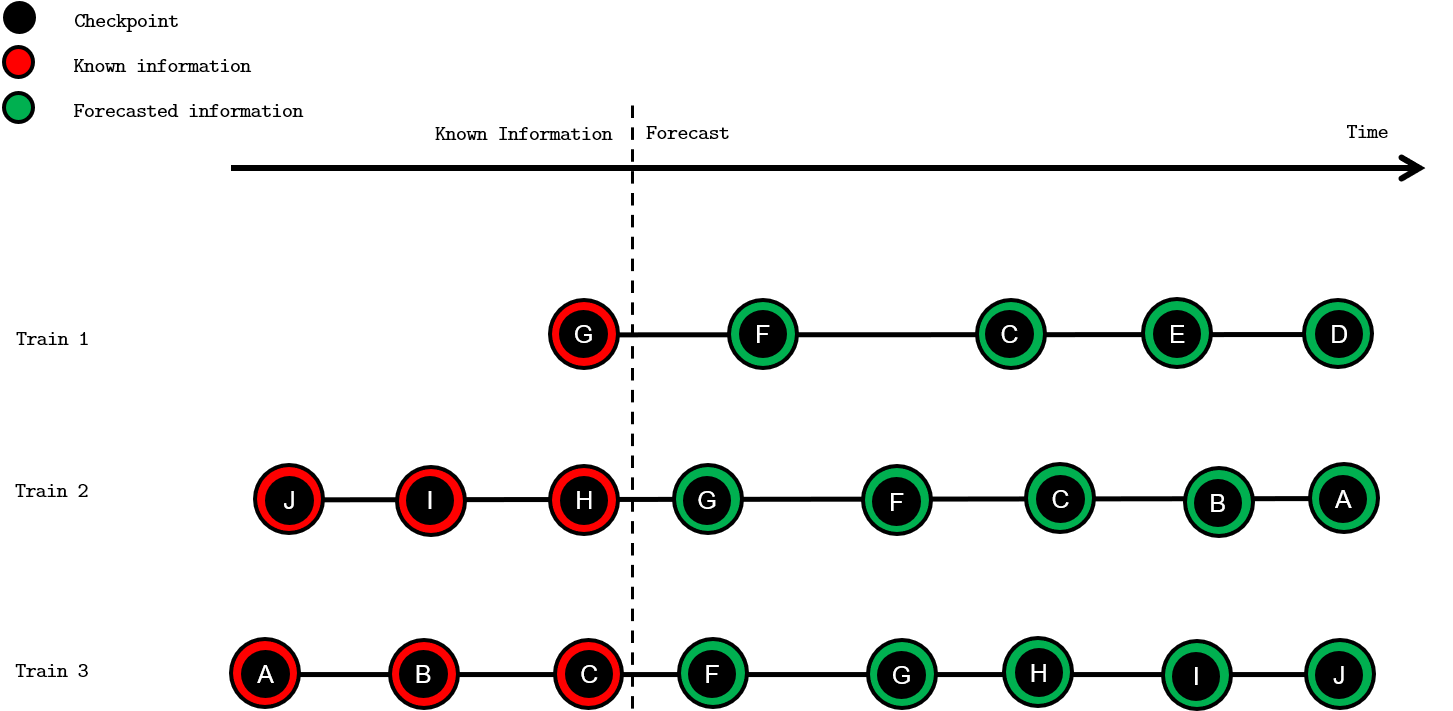
\includegraphics[width=\textwidth]{Images/ForecastProblem.png}}}
\caption{Forecasting schematic of 3 example trains} \label{ForecastProblem}
\end{figure}

\subsection{Delay Propagation Mechanisms}\label{subsection:delay_propagation_mechanisms}
We adopt five key delay propagation mechanisms focused on how the delay of an example train, Train 1 travelling from station A to Station B propagates to some Train 2, with the exception of delay propagation mechanism 1 which concerns train 1 exclusively.

Delay propagation mechanism 1 - self propagation. The arrival delay of Train 1 to station B resulting in the departure delay of Train 1 departing from station B, $D_{C_i}^{Train 1} = f(A_{C_i}^{Train 1})$.
\begin{figure}[H]
\centering
{%
{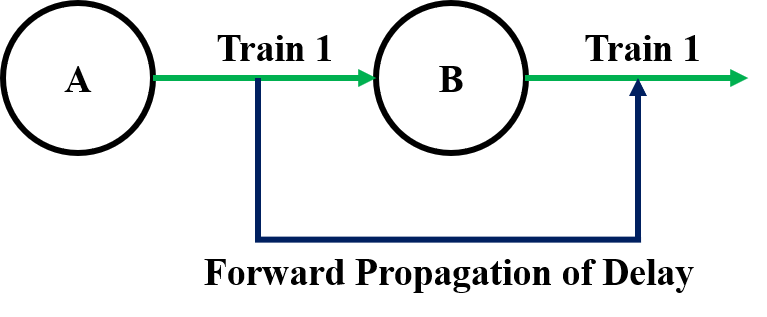
\includegraphics[width=0.5\textwidth]{Images/SelfDepartureForwardPropagation.png}}}
\caption{Self Forward Delay Propagation} \label{SelfDepartureForwardPropagation}
\end{figure}

Delay propagation mechanism 2 - arrival backward delay propagation. The departure delay of Train 1 from station A resulting in the arrival delay of Train 2 at station A, $A_{C_i}^{Train 2} = f(D_{C_i}^{Train 1})$.
\begin{figure}[H]
\centering
{%
{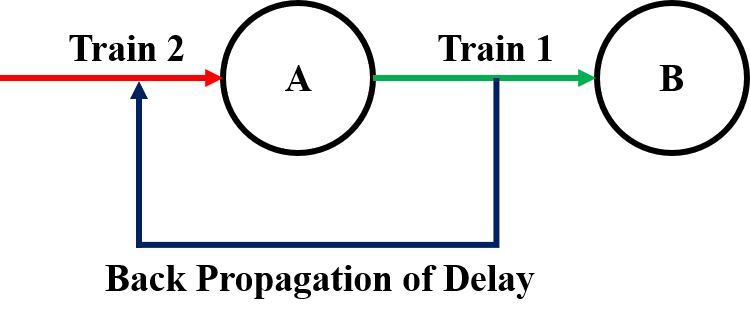
\includegraphics[width=0.5\textwidth]{Images/ArrivalBackwardPropagation.png}}}
\caption{Arrival Backward Delay Propagation} \label{ArrivalBackwardPropagation}
\end{figure}

Delay propagation mechanism 3 - arrival forward delay propagation. The arrival delay of Train 1 at station B resulting in the arrival delay of Train 2 at station B, $A_{C_i}^{Train 2} = f(A_{C_i}^{Train 1})$.
\begin{figure}[H]
\centering
{%
{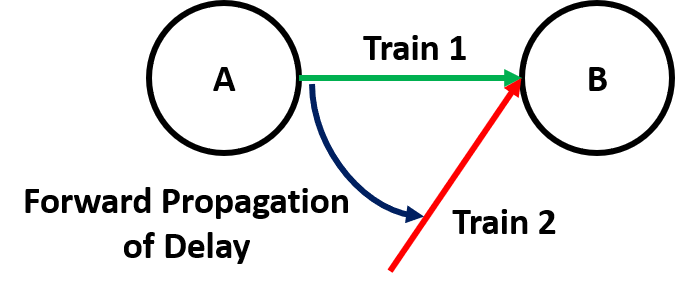
\includegraphics[width=0.5\textwidth]{Images/ArrivalForwardPropagation.png}}}
\caption{Arrival Forward Delay Propagation} \label{ArrivalForwardPropagation}
\end{figure}

Delay propagation mechanism 4 - departure backward delay propagation. The departure delay of Train 1 from station A resulting in the departure delay of Train 2 from station A, $D_{C_i}^{Train 2} = f(D_{C_i}^{Train 1})$.
\begin{figure}[H]
\centering
{%
{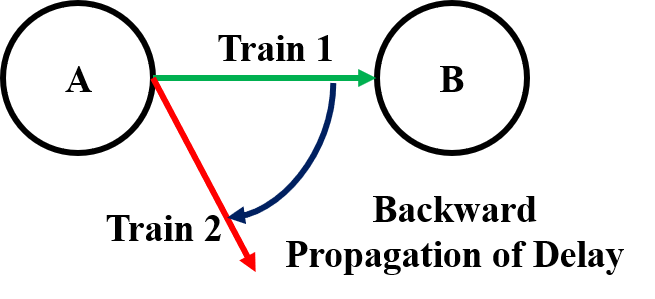
\includegraphics[width=0.5\textwidth]{Images/DepartureBackwardPropagation.png}}}
\caption{Departure Backward Delay Propagation} \label{DepartureBackwardPropagation}
\end{figure}

Delay propagation mechanism 5 - departure forward delay propagation. The arrival delay of Train 1 at station B resulting in the departure delay of Train 2 from station B, $D_{C_i}^{Train 2} = f(A_{C_i}^{Train 1})$.
\begin{figure}[H]
\centering
{%
{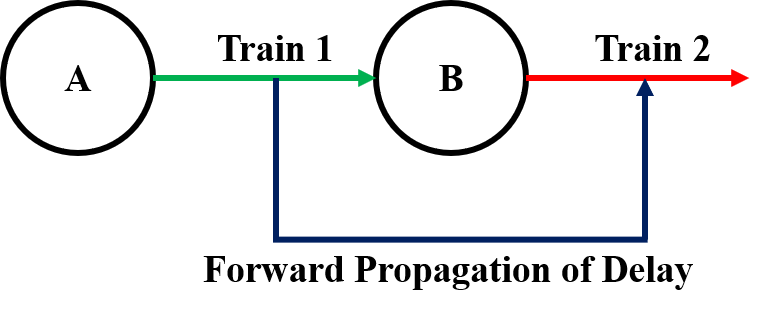
\includegraphics[width=0.5\textwidth]{Images/DepartureForwardPropagation.png}}}
\caption{Departure Forward Delay Propagation} \label{DepartureForwardPropagation}
\end{figure}

\subsection{The Deep Neural Network Model}\label{DNNSubsection}

A DNN is a hierarchical model where each layer uses the output of the previous layer as its input and is based on unsupervised learning of multiple levels where higher level features are derived from the lower level features. Each layer in the neural network is made up of neurons. The input layer of the DNN shall represent the input matrix, the output layer representing the predictions. Hidden layers are those in between the input and output layer. Iterative gradient methods are used to train the neural network. Repeatedly, weights are assigned to each neuron to progressively make predictions on the subset of the data in a forward pass manner. Each neuron receives weighted input variables from the outputs of the neurons connected to it in the previous layer, and in response, a set of predetermined functions are performed on these values to produce an output to be sent the connecting neurons in the next layer. Upon the completion of the forward pass procedure, the loss function $L$ is calculated and updated weighted values $w$ proportional to $dL/dw$ are formed. This process of forwards and backwards propagation is repeated until a stopping criterion is met.

\subsection{The Extreme Gradient Boosting Model}\label{XGBoostSubsection}
The gradient boosting technique is an ensemble learning method whereby trees are sequentially built, aiming to reduce the errors of the previous tree. For a sample set of $\{(x_1,y_1),...,(x_N,y_N)\}$ with explanatory variables $\boldsymbol{X}$ and $Y$ response variables, an initial model $F_0(\boldsymbol{X})$ is defined to predict the response variables, $\hat{y}_0$, by minimizing the differentiable convex loss function $l(y,F_0(\boldsymbol{X}))$. The gradient of the loss function, $r_0$ is then computed and fitted with a new regression tree $h_1$. The first boosted model, $F_1(\boldsymbol{X})$, is then computed through a combination of weighted regression trees and the previous model. This process is repeated for M iterations until a stopping condition has been reached. The Extreme Gradient boosting framework (XGBoost) is a supervised ensemble learning method based on ensemble trees and follows the gradient boosting principles however utilizes a more regularized model to minimize over-fitting. Having \textit{K} trees, the prediction, $\hat{y}_i$ can be represented by the following function:
\begin{equation}
    \hat{y_i} = \phi(x_i)=\sum_{k=1}^{K}h_k(x_i), \; h_k \in H
\end{equation}
or similarly, the prediction at the $m^{th}$ step is defined as:
\begin{equation}
    \hat{y_i}_m = \phi(x_i)_m=\sum_{k=1}^{m}h_k(x_i), \; h_k \in H
\end{equation}
where, $\hat{y_i}$ is the predicted values, $H$ is the set of all possible regression trees and $h_k$ is the k\textsuperscript{th} regression tree that is learned through minimizing the following cost objective function at step m:
\begin{equation}\label{XGBoostObj}
    L(\theta)_m = \sum_{i=1}^{N}l(y_i,\hat{y}_{im}) + \sum_{i=1}^{m}\Omega(h_i) = \sum_{i=1}^{N}\left[l(y_i,\hat{y}_{i(m-1)})+ h_m(x_i)\right] + \sum_{i=1}^m\Omega(h_i)
\end{equation}

Through utilizing the Taylor expansion, the cost objective function can be approximated to be:
\begin{equation}
    L(\theta)_m = \sum_{i=1}^{N}\left[l(y_i,\hat{y}_{i(m-1)}) + g_i h_m(x_i) + \frac{1}{2}h_i h^2_m(x_i)\right] + \sum_{i=1}^m\Omega(h_i)
\end{equation} 
where
\begin{equation}
    g_i = \partial{\hat{y}_{i(m-1)}}l(y_i,\hat{y}_{i(m-1)})
\end{equation} 
\begin{equation}
    h_i = \partial^2{\hat{y}_{i(m-1)}}l(y_i,\hat{y}_{i(m-1)})
\end{equation} 
$\Omega(h_i)$ is the regularization term in the form of a penalty that increases with the complexity of the ensemble $H$ in order to avoid over-fitting. For the XGBoost algorithm, the penalty relates to the number of leaves per tree $T$, regression tree score $w_j$ at each leaf and hyper-parameters $\gamma$ and $\lambda$ as portrayed below:

\begin{equation}
    \Omega(h) = \gamma T + \frac{1}{2}\lambda \sum_{j=1}^{T}w_j^2
\end{equation} 
At each step $m$, the algorithm greedily adds the hypothesis $h_m$ that best minimizes that objective. 

\subsection{The Data} \label{PreprocessingSection}
The data utilized in this paper is provided through Darwin. Specifically, the application programming interface (API) utilized is the historical service performance (HSP) API \citep{NRE19}. This API provides two data sets through two separate calls in Javascript Object Notation (JSON) Format that shall be used in conjunction with each other, Service Metrics –-- requiring the origin and destination stations, first departure and final arrival times and start and end dates to be defined as inputs and Service Details –-- requiring train IDs provided by the Service metrics API as input. The data received through the Service Metric call is outlined in Table \ref{ServiceMetrics} and data received through the Service Details call is outlined in Table \ref{ServiceDetails}.

\begin{table}[H]
\tbl{Service metrics provided by Darwin's HSP}
{\begin{tabular}{ll} 
 Key  &  Description\\ \midrule
 Origin Location  &  Computer Reservation System (CRS) Code of Origin\\
 Destination Location  &  CRS code of destination\\
 gbtt ptd  &  Scheduled Public departure time at departure station\\
 gbtt pta  &  Scheduled Public arrival time at destination station\\
 TOC code  &  Code of train operating company\\
 RIDs  &  Train ID\\
 Matched services  &  List of all train RIDs \\
 Tolerance Value  &  Selected tolerance value\\
 Num not tolerance  &  Number of trains outside the tolerance\\
 Num tolerance  &  Number of trains within the tolerance\\
 \bottomrule
\end{tabular}}
\label{ServiceMetrics}
\end{table}

\begin{table}[H]
\tbl{Service details provided by Darwin's HSP}
{\begin{tabular}{ll} 
 Key  &  Description\\ \midrule
 Date of service  &  Date of service of the specified train RID\\
 TOC Code  &  Code of train operating company\\
 RID  &  Inputted RID\\
 Location  &  CRS code of train location\\
 gbtt ptd  &  Scheduled Public departure time\\
 gbtt pta  &  Scheduled Public arrival time\\
 Actual td  &  Actual departure time\\
 Actual ta  &  Actual arrival time\\
 Late canc reason  &  Code that specifies late or cancellation reason\\
 \bottomrule
\end{tabular}}
\label{ServiceDetails}
\end{table}


All time values provided by Darwin’s service details API are accurate to the nearest minute and include all origin-destination trips that pass through the allocated origin and destination stations. For this paper, Didcot Parkway and London Paddington were selected as the gateway stations; i.e., all train journeys that include both these stations in their schedule in both inbound and outbound directions are included in the dataset. Journeys between these stations are the choice of this paper due to its notoriety in providing prevalent delayed services \citep{DFT16}. All train journeys between 06:00 am and 10:00 am from 2016 shall be used in training the ML models while all train journeys between 06:00 am and 10:00 am in 2017 data shall be used to test the ML models. This time range was selected to capture the mechanics of delay propagation amidst morning rush hour and hence, peak usage. The days used to train this model have been specified as non-holiday weekdays. The day, month, order of train departure, origin departure period and current train checkpoint adds temporal dimensions to the model whereas all other variables add spatial dimensions to the model. In the inbound direction, Darwin provides 10,767 journeys in 2016 and 10,742 journeys in 2017 initiating at various stations, passing through Didcot Parkway and terminating at London Paddington. In the outbound direction, Darwin provides 9,069 journeys in 2016 and 8,969 journeys in 2017 initiating at London Paddington and passing through Didcot Parkway to their respective destination stations. According to the Office of Rail and Road (ORR), 505,215 Great Western Railway journeys were planned in 2016 and 532,501 in 2017 \citep{ORRGWR19}. Therefore, our ML models are trained on 4\% of all Great Western Railway Journeys in 2016 and tested on 3.7\% of all Great Western Railway Journeys in 2017. Figure \ref{Schematic} portrays all the checkpoints considered in this paper. 

\begin{figure}[h!]
\centering
{%
{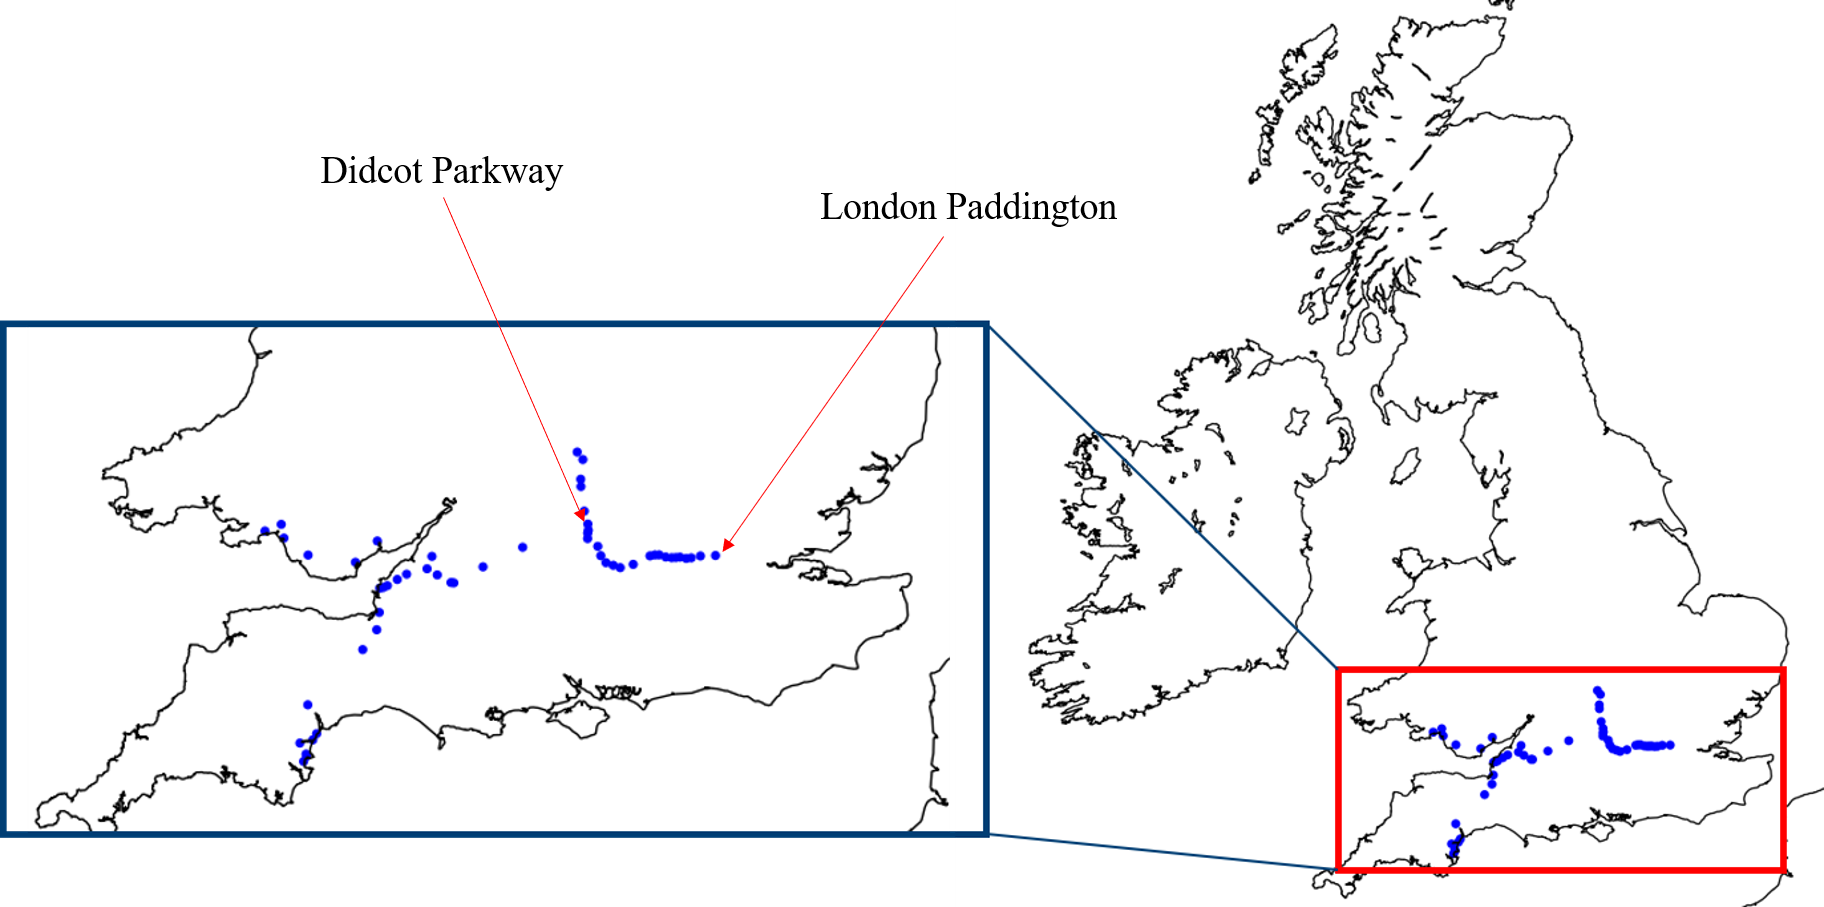
\includegraphics[width=\textwidth]{Images/Schematic.png}}}
\caption{Figure illustrating all checkpoints considered in this paper} \label{Schematic}
\end{figure}

\subsection{Data Preprocessing}
The dataset provided by Darwin's HSP API underwent preprocessing and feature engineering in order to produce an input space that best outlines the context of the problem per Section \ref{ProblemFormulationSection}, therefore ensuring the best performance of the XGBoost and DNN models outlined in Sections \ref{XGBoostSubsection} and \ref{DNNSubsection}. 
The data that shall be used in the models of this paper is processed by looping through Darwin's Service Metrics and Service Details API to achieve the spatial and temporal constraints outlined in section \ref{PreprocessingSection}. Missing information was of primary concern and was dealt with before any features were engineered. All missing information in this paper originate from the 'actual\_td' and the 'actual\_ta' categories of Darwin's Service Details API, that is the actual departure time and arrival time of a train at a station respectively due to the nature of data collection, in this case through sensors. In order to account for this missing data issue we apply the practice to dismiss any train journey data that have more than 10\% missing data.  
When there is less than 10\% missing data, sample imputation shall be used. The average actual and average planned travel times between two unique station pairs and the average dwell time of each unique station are evaluated and utilized to fill in the missing arrival and departure times. Following the missing data imputation process, feature engineering is performed to produce the input space, $\boldsymbol{X} \in \mathbb{R}^{n \times p}$, where $n$ is the number of data points and $p$ is the number of input features for the models in this paper. These features and the processes undertaken to produce them are outlined in Section \ref{SubSection:FeatureEngineering}.

\subsection{Hyper-Parameter Optimization}
This section shall explain and justify the architectural configuration of the DNN and XGBoost models used in this paper. The DNN model is built using the Keras deep learning python library \citep{chollet2015keras} and the XGBoost model is built using the XGBoost python package. Any learning algorithm, $A$, is made of a set of hyper-parameters, $\boldsymbol{\lambda}$, the purpose in fine-tuning $\boldsymbol{\lambda}$ is to produce an optimal $A$ that minimizes the expected loss of the model $L$. Although currently, there is no superior global algorithm to find the optimal set of hyper-parameters, several techniques exist such as the grid searching cross-validation, randomized search cross-validation and genetic algorithms. This paper shall utilize the grid search cross-validation technique through scikitlearn \citep{scikit-learn}. 

\subsubsection{DNN}
For the DNN model, all combinations of all hyper-parameter values detailed in Table \ref{table:OneStepPrediction}, are tested to reach a global optimal configuration. Table \ref{table:DNNHPFixed} details hyper-parameters that were not fine-tuned due to reasons detailed in the description.
\begin{table}[H]
\tbl{Summary of DNN hyper-parameter fine-tuning}
{\begin{tabular}{p{0.3\textwidth}ccp{0.6\textwidth}}\hline
Hyper-parameter  &  Values(s)  &  Optimum  &  Description \\ \hline
Batch Size  &  50, 100  &  100  &  The number of examples that are utilized in each iteration before the neural network's parameters are updated. A large batch size reduces the training time; however, this may cause accuracy loss \citep{SAM17}. \\ 
Epoch  &  50, 100, 150  &  50  &  The number of times the algorithm completes forwards and backwards pass of all training examples. A larger epoch number risks over-fitting but a smaller epoch number risk lower accuracy.\\ 
Drop-out  &  0, 0.2  &  0.2 &  The drop-out algorithm is used to combat over-fitting. A value too small may still induce over-fitting whereas a value too large may hinder the model's learning process. \\ 
Number of hidden layer neurons  &  10, 18, 25  &  18  &  A value too small fails to convey the information of the input neurons whereas a value too large will increase processing times.  \\ 
Number of hidden layers  &  1, 2, 3  &  2  &  A value too small fails to convey the information of the input neurons whereas a value too large will increase processing times. \\ 
\bottomrule
\end{tabular}}
\label{table:OneStepPrediction}
\end{table}


\begin{table}[H]
\tbl{Summary of Fixed DNN hyper-parameters}
{\begin{tabular}{p{0.3\textwidth}ccp{0.6\textwidth}}\hline
Hyper-parameter  &  Values(s)  &  Optimum  &  Description \\ \hline
Optimization Algorithm  &  Adam  &  -  &  The optimization algorithm was not varied since it does not have a direct effect in improving the model accuracy as much as how fast the model takes to converge. It has been empirically proven that the optimization algorithm 'Adam' outperforms other algorithms in a neural network \citep{KIN14}.\\ 
Network Weight Initialization  &  Random Normal  &  -  &  The weight initializer is set as random normal (mean of 0 and standard deviation of 0.5) since the input parameters of the model are normalized and scaled relative to each other theoretically meaning faster convergence with this method. \\ 
Neuron Activation Function  &  ReLU  &  -  &  This activation function is used as convergence is reached significantly faster than other activation functions \citep{KRI12}\\
\bottomrule
\end{tabular}}
\label{table:DNNHPFixed}
\end{table}
\subsubsection{XGBoost}
For the XGBoost model, we applied fine-tuning to the maximum depth of tree and the minimum sum of instance weight needed in a child (minimum child weight), regarded as the two most important hyperparameters dictating model performance as well as the learning rate and the number of trees. The details regarding these parameters are in Table \ref{table:OneStepPredictionXGBoost}.

\begin{table}[H]
\tbl{Table detailing the XGBoost model's variables fine-tuned for the one-step prediction}
{\begin{tabular}{p{0.4\linewidth}ccp{0.5\linewidth}}\hline
Hyper-parameter  &  Value(s)  &  Optimum  &  Description \\\hline
Learning Rate  &  0.01, 0.1  &  0.1  &  Generally, the learning rate is best kept as 0.1, however, if the learning rate were to be increased, then the number of trees would be reduced and vice versa. \\ 
Number of trees  &  100, 200, 300  &  300  &  The default number of trees provided by the XGBoost package is set as 100. \\ 
Maximum depth of tree  &  3, 5, 7, 9  &  5  &  By increasing this value, the model's complexity will increase however, over-fitting must be considered.  \\ 
Minimum sum of instance weight needed in a child  &  1, 3, 5  &  1  &   A larger value results in a more conservative model. \\
\bottomrule
\end{tabular}}
\label{table:OneStepPredictionXGBoost}
\end{table}

\subsection{Feature Engineering}\label{SubSection:FeatureEngineering}
All historical data provided by Darwin's HSP underwent an initial feature engineering process to extract the features summarized in Table \ref{InputFeatureTable}.

\begin{table}[H] 
\tbl{Feature engineering summary}
{\begin{tabular}{cp{6cm}p{10cm}}\hline
 Feature  &  Input Parameter  &  Feature Summary\\ \hline
 1  &  Cumulative arrival delay of train journey up to $C_i$  &  $\sum_{i=0}^{i}A_{C_i}$ \\ 
 2  &  Cumulative departure delay of the train journey up to $C_i$  &  $\sum_{i=0}^{i}D_{C_i}$\\ 
 3  &  Day  &  Provided by HSP\\ 
 4  &  Arrival delay, $A_{C_i}$, of the train at the current checkpoint  &  $TA_{C_i}-TA\textprime_{C_i}$\\ 
 5  &  Departure delay, $D_{C_i}$, of the train at the current checkpoint, this also represents delay type 1 - self propagation  &  $TD_{C_i}-TD\textprime_{C_i}$\\  
 6  &  Delay Type 2 - Arrival backward delay propagation &  $A_{C_i}^{Train 2} = f(D_{C_i}^{Train 1})$\\  
 7  &  Delay Type 3 - Arrival  forward  delay  propagation & $A_{C_i}^{Train 2} = f(A_{C_i}^{Train 1})$\\  
 8  &  Delay Type 4 - Departure backward delay propagation &  
$D_{C_i}^{Train 2} = f(D_{C_i}^{Train 1})$\\  
 9  &  Delay Type 5 - Departure forward delay propagation &  $D_{C_i}^{Train 2} = f(A_{C_i}^{Train 1})$\\ 
 10  &  Direction of travel  &  \\ 
 11  &  Dwell time, $DT$, of the train at the current checkpoint  &  $TD_{C_i}-TA_{C_i}$\\ 
 12  &  Average dwell time of all trains at station $C_{i+q}$, $q=\{1,...,10\}$  &  Deduced from unique station dwell time\\ 
 13  &  Whether or not the current station is the origin station  &  Self explanatory\\ 
 14  &  Whether or not the current station is the terminating station  &  Self explanatory\\ 
 15  &  Month  &  Provided by HSP\\ 
 16  &  Number of stops  &  Provided by HSP\\ 
 17  &  Order of departure from the origin station of the train on the day of its journey relative to other trains  &  ll individual journeys in a day are ranked\\ 
 18  &  What stop the train is at with respect to its journey  &  Self explanatory\\ 
 19  &  Origin departure period  &  Split up into four categories, if the train departed from its original station from 06:00 and 07:00, then $\chi_{15}=0$, if its departure is between 07:00, $\chi_{15}=2$ and finally, 09:00 and 10:00, $\chi_{15}=3$\\ 
 20  &  Average travel time from the $C_{\text{Prediction}-1}$ to $C_{\text{Prediction}}$  &  Deduced from average travel time between unique OD pairs\\ 
 21  &  Travel time from the previous checkpoint to the current checkpoint $TT_{C_{i-1},C_{i}}$  &  $TA_{C_i}-TD_{C_{i-1}}$\\
 \bottomrule
\end{tabular}}
\label{InputFeatureTable}
\end{table}

In order to make the engineered data compatible with the ML models, we processed the data further. We transformed all train journeys as provided by Darwin, and following the feature engineering process, we encoded nominal categorical parameters, specifically features 3 - day, 6 - direction of travel, 9 - whether or not the current station is the origin station, 10 - whether or not the current station is the terminating station and 11 - month. As is the nature of nominal categorical data, their representation must not convey ordinality, therefore, we created dummy variables and omitted one dummy variable as to avoid perfect collinearity or the "dummy variable trap" in the prediction process. Finally, we standardized each feature $x_i$ independently through centering and scoring using the mean $\mu$ and variance $\sigma$ as shown in Equation \ref{Equation:ScaleScore}. Table \ref{table:FinalInputKey} shall hereafter, be used as reference for the input variable. Note that the input space for the models are derived from actual information upon the departure of train $k$ from station $C_i$ i.e. all data engineered for the input space for the ML models correspond to data from accumulated for a train $k$ up and prior to the train departing from station $C_i$. 

\begin{equation}
    Z = \frac{x_i-\mu}{\sigma}
\label{Equation:ScaleScore}
\end{equation}

\begin{table}[H]
\tbl{Final input variable matrix}
{\begin{tabular}{clcl}\hline
Feature No. & Feature & Feature No. & Feature \\ \hline
1 & Tuesday & 18 & Arrival Delay at Current Checkpoint\\
2 & Wednesday & 19 & Departure Delay at Current Checkpoint\\
3 & Thursday & 20 & Delay Type 2 - Arrival backward delay propagation\\
4 & Friday & 21 & Delay Type 3 - Arrival forward delay propagation\\
5 & February & 22 & Delay Type 4 - Departure backward delay propagation\\
6 & March & 23 & Delay Type 5 - Departure forward delay propagation\\
7 & April & 24 & Direction of Travel \\
8 & May & 25 & Dwell Time at Current Checkpoint\\
9 & June & 26 & Average Dwell Time at Predicted Station\\
10 & July & 27 & Origin Station\\
11 & August & 28 & Terminal Station\\
12 & September & 29 & Number of Stops\\
13 & October & 30 & Scheduled Order of Departure Of the Day\\
14 & November & 31 & Current Checkpoint of the Train Journey\\
15 & December & 32 & Origin Departure Period\\
16 & Cumulative Arrival Delay & 33 & Average Travel Time from the Checkpoint before the predicted to the predicted Checkpoint\\
17 & Cumulative Departure Delay & 34 & Travel Time from previous check point to Current Checkpoint\\
\bottomrule
\end{tabular}}
\label{table:FinalInputKey}
\end{table}

The actual output space $Y^A$ and forecasted output space $Y^F$ for each journey of each train $k$ at each checkpoint $C_i$, composes of, actual and forecasted time travelled from the station $C_{i+q-1}$ to station $C_{i+q}$, i.e. $TT_{C_{i+q-1},C_{i+q}}$ and $\hat{TT}_{C_{i+q},C_{i+q-1}}$ respectively, actual and forecasted dwell time at station $C_{i+q}$, i.e. $DT_{C_{i+q}}$ and $\hat{DT}_{C_{i+q}}$ respectively, actual and forecasted arrival delay at station $C_{i+q}$, i.e. $A{C_{i+q}}$ and $\hat{A}{C_{i+q}}$ respectively and actual and forecasted departure delay at station $C_{i+q}$, i.e. $D_{C_{i+q}}$ and $\hat{D}_{C_{i+q}}$. In this paper, KPIs of up to ten future checkpoints relative to the train’s current checkpoint shall be predicted, i.e. $q \in \{1,2,...,10\}$. Hence, ten models shall be trained through the DNN and XGBoost frameworks each. During the training stage, if the future prediction step $q$ is greater than the number of checkpoints left within the train’s particular journey the output space is set to be 0. If the number of checkpoints left within the train’s particular journey is equal to the number of remaining checkpoints, only the dwell time and departure departure delay predictions are set to be 0.

\section{Results and Evaluation}\label{ResultsAndEvaluationSection}
To ensure an unbiased evaluation of the predictive capabilities of the DNN and XGBoost models, careful consideration is required in selecting performance metrics. Due to the nature of the predictions made by the models of this paper encompassing near-zero values, we decided that the standard performance metric, the mean absolute percentage error (MAPE) or the symmetrical mean and absolute percentage error (SMAPE) shall not be utilized to evaluate performance due to these metrics' setbacks in dealing with near zero values. Instead, we propose utilizing the mean arctangent absolute percentage error term  (MAAPE) developed by \citeauthor{KIM16} (\citeyear{KIM16}) that allows for improved symmetry compared to MAPE, but most importantly, the ability to assess near-zero values that render MAPE and SMAPE to infinity. We shall also utilize the root mean square error (RMSE) and the coefficient of determination, $r^2$ and the average absolute error for each variable of the output space $\boldsymbol{Y}$, ATTAE (average travel time absolute error), AADAE (average arrival delay absolute error), ADDAE (average departure delay absolute error) and ADTAE (average dwell time absolute error) to evaluate our models' performances.These metrics are illustrated in Equations \ref{Equation:RMSE} to \ref{Equation:ADTAE}. It should be noted that whilst the models were trained using all data available, we shall not evaluate predictions of all trains that do not experience a delay in departure from its most recent checkpoint from the evaluation. This is because the aim of this research is to produce models that predict train KPIs following a delay and the inclusion all train movements in the frameworks provide information on primary delays that are vital in the prediction of subsequent KPIs. We also compared the performance of DNN and XGBoost models with the standard multiple linear regression model as well as a decision tree model. This was done to demonstrate and benchmark the DNN and XGboost models' superior predictive capabilities. It is useful to note that, using an Intel(R) Core(TM) i7-7700HQ CPU at 2.80GHz, our DNN models took, on average, 58.95 seconds to train, whereas our XGBoost models took, on average, 80.44 seconds to train, these times are broken down further into their respective step considerations in Table \ref{tab:XGBTrainTime}. 

\begin{equation}\label{Equation:RMSE}
   RMSE = \sqrt{\frac{\sum_{j=1}^{n}(Y^F_j-Y^A_j)^{2}}{n}}
\end{equation}
\begin{equation}\label{Equation:R2}
    r^2 = 1 - \frac{\sum_{j=1}^{n}(Y^A_j - Y^F_j)^2}{\sum_{j=1}^{n}(Y^A_j-\frac{1}{n}\sum_{j=1}^nY^A_j)^2} 
\end{equation}
\begin{equation}\label{Equation:MAAPE}
   MAAPE = \frac{\sum_{j=1}^{n}\text{arctan}\left(\left|\left|\frac{Y_j^{A}-Y_j^{F}}{Y_j^{A}}\right|\right|\right)}{n} 
\end{equation}
\begin{dblequation}\label{Equation:ATTAE}
    ATTAE  = \frac{\sum_{j=1}^{n}TTAE_j}{n}, & TTAE_j = ||\hat{TT}_{C_{j+q},C_{j+q-1}}-TT_{C_{j+q},C_{j+q-1}}||
\end{dblequation}
\begin{dblequation}\label{Equation:AADAE}
     AADAE  = \frac{\sum_{j=1}^{n}{ADAE}_j}{n}, & ADAE_j  = ||\hat{A}_{C_{i+q}}-{A}_{C_{i+q}}||
\end{dblequation}
\begin{dblequation}\label{Equation:ADDAE}
     ADDAE  = \frac{\sum_{j=1}^{n}{DDAE}_j}{n}, & DDAE_j  = ||\hat{D}_{C_{i+q}}-{D}_{C_{i+q}}||
\end{dblequation}
\begin{dblequation}\label{Equation:ADTAE}
     ADTAE  = \frac{\sum_{j=1}^{n}{DTAE}_j}{n}, & DTAE_j  = ||\hat{DT}_{C_{i+q}}-{DT}_{C_{i+q}}||
\end{dblequation}
\normalsize

\subsection{Model Results}\label{Subsection:ModelResults}
\begin{figure}[H]
     \centering
     \subfloat[][DNN]{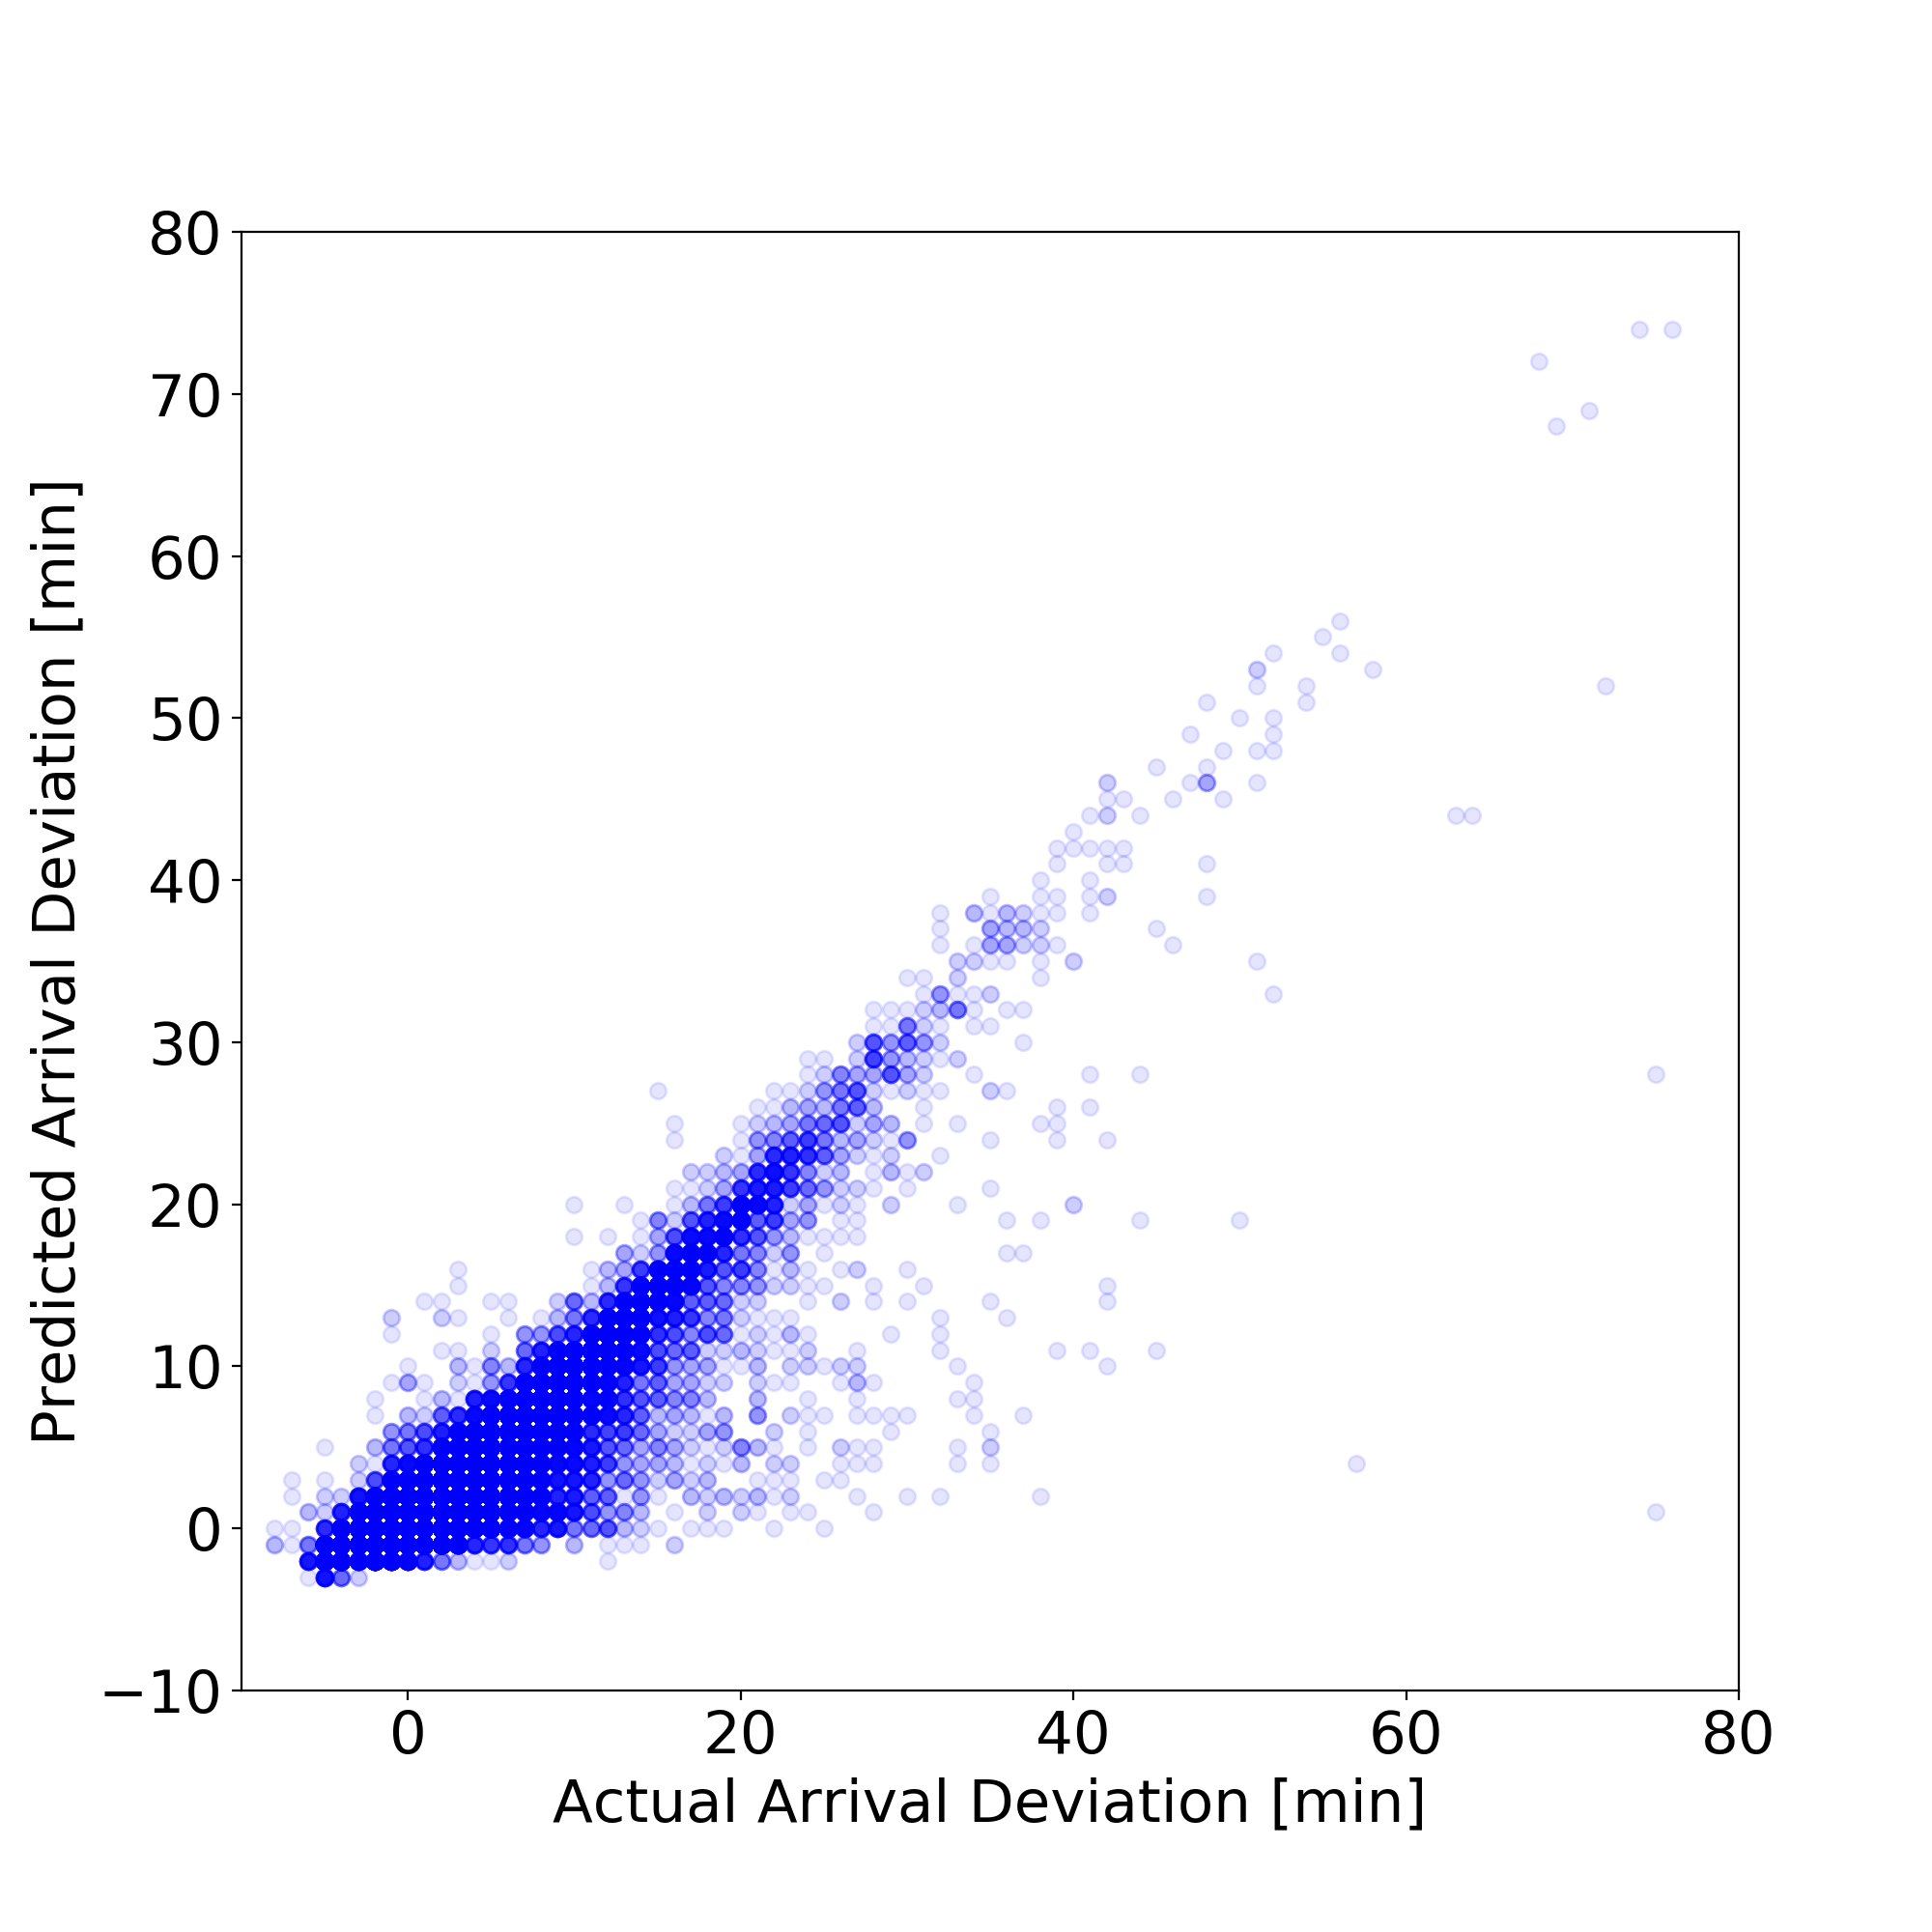
\includegraphics[width=0.5\textwidth]{Images/DNN_plot/1_step/1_step_arrival_deviation.png}}
      \subfloat[][XGBoost]{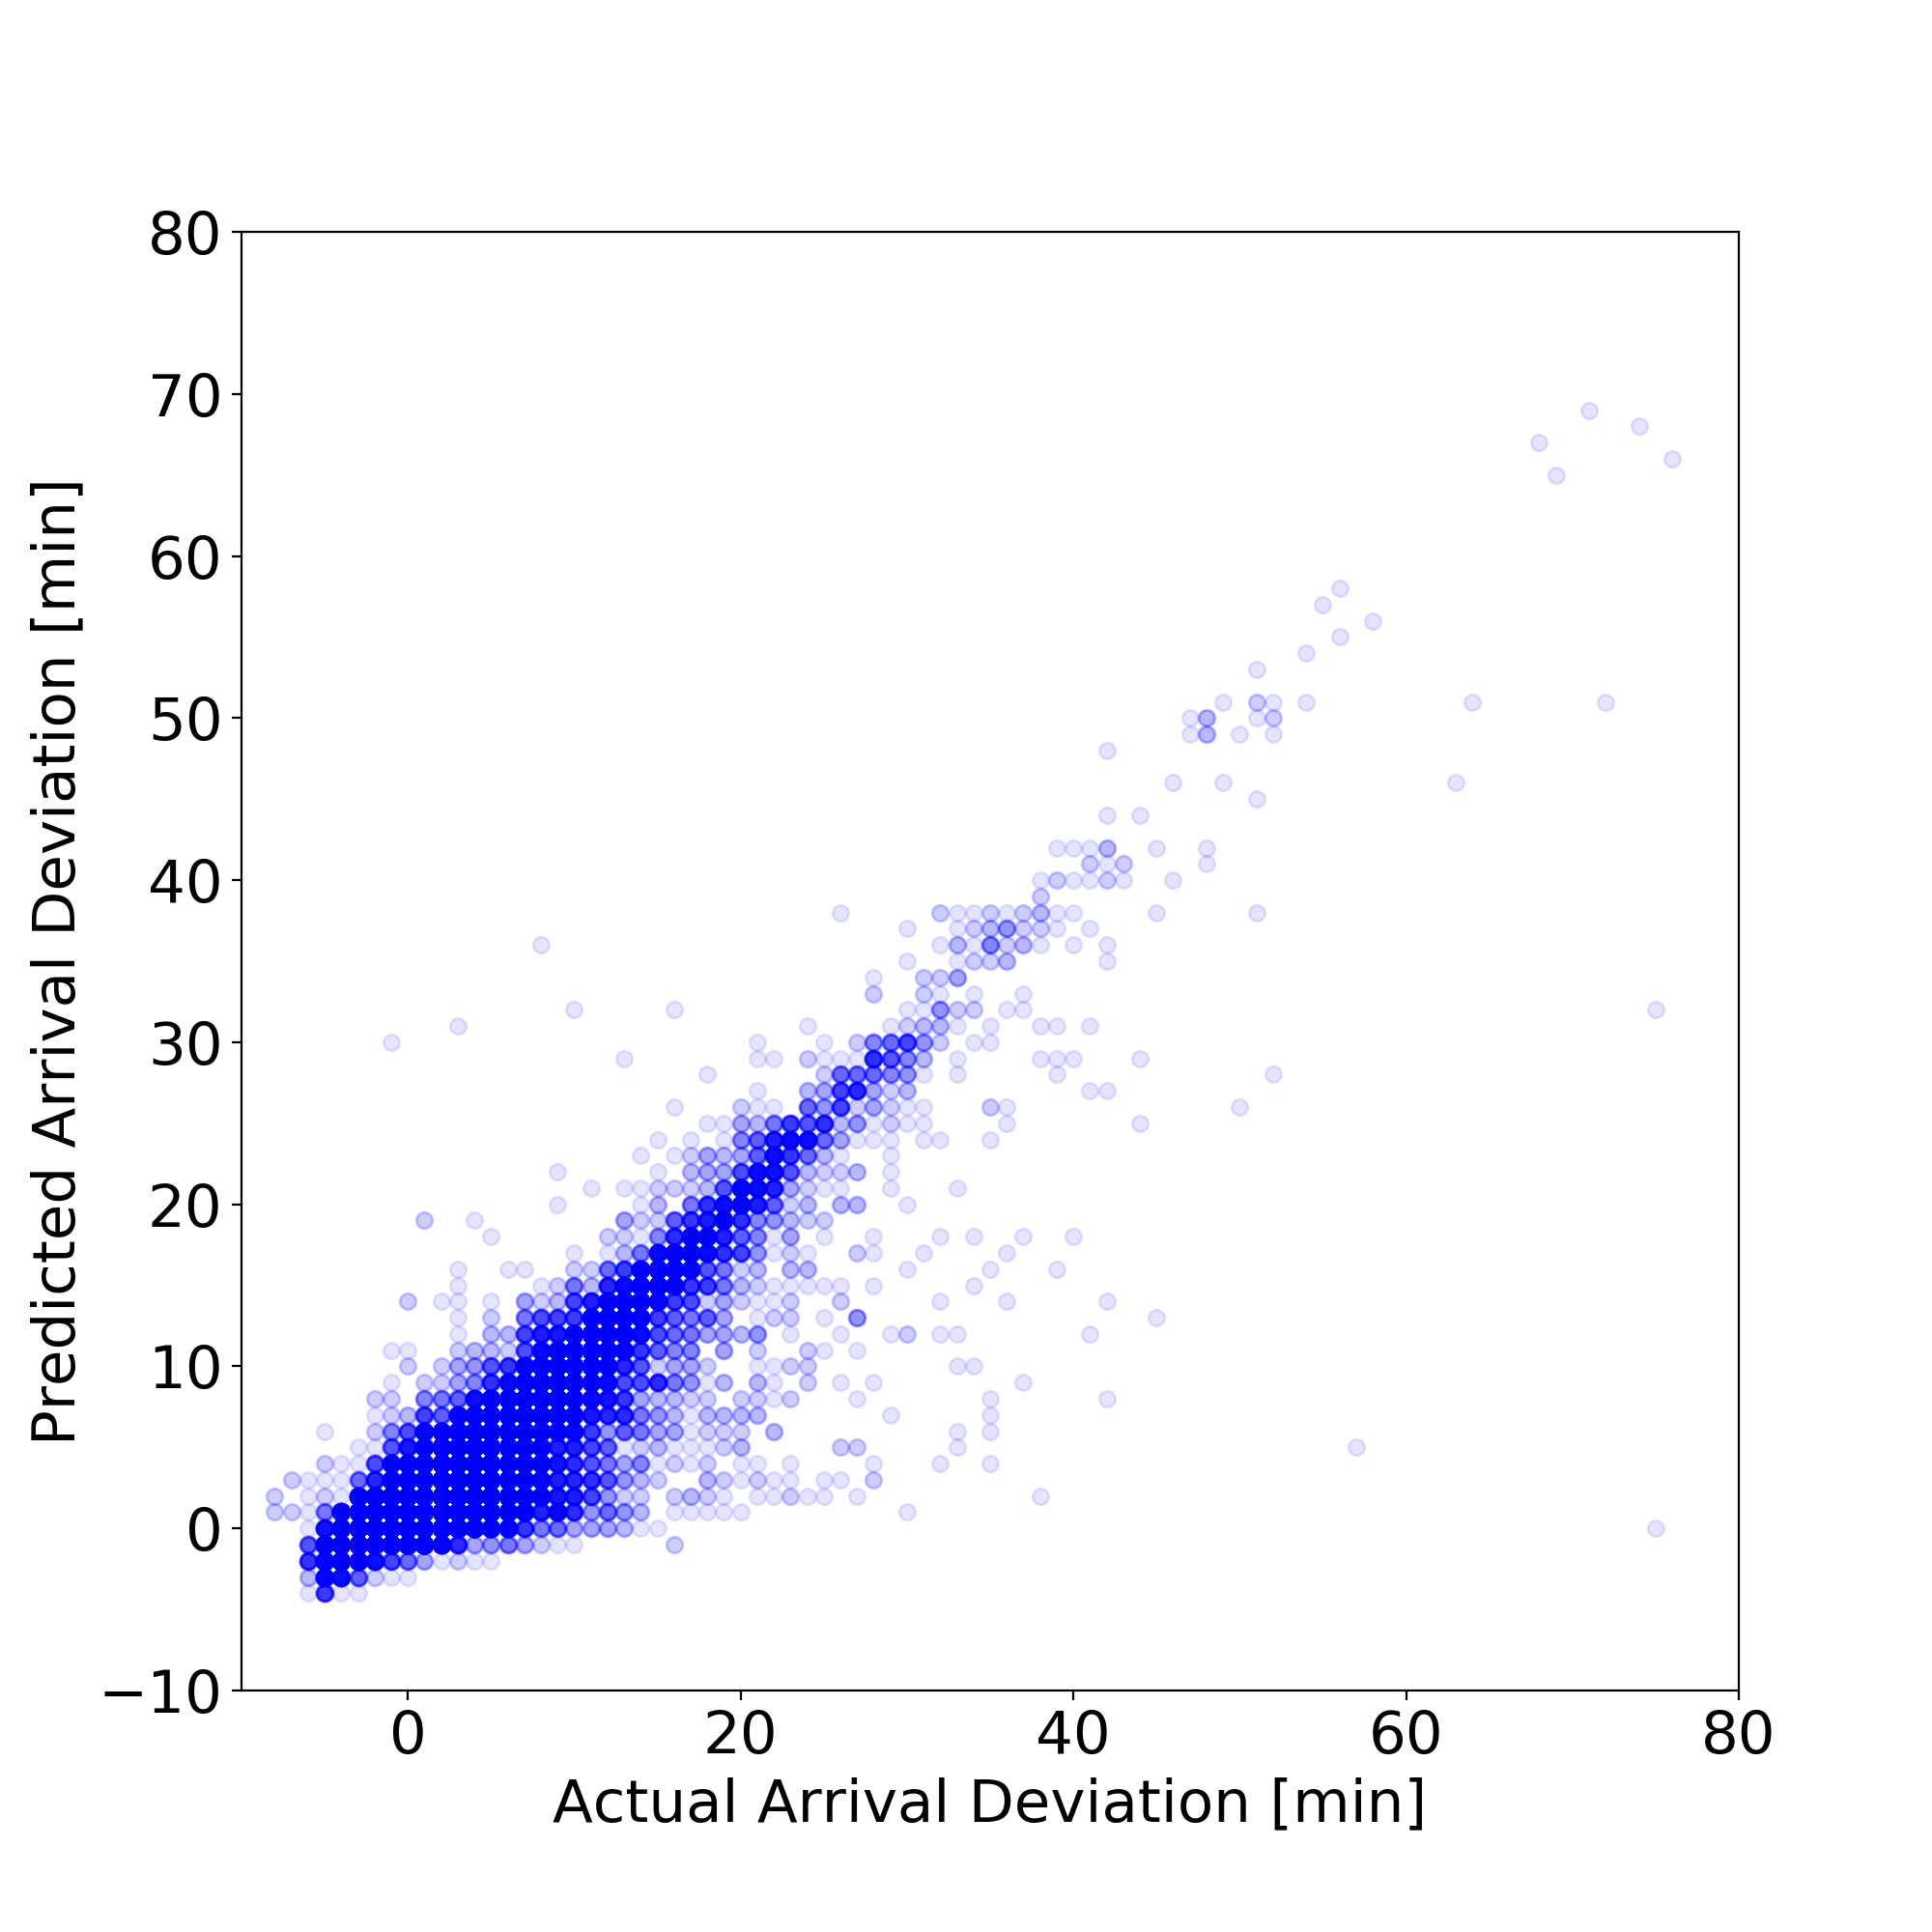
\includegraphics[width=0.5\textwidth]{Images/XGBoost_plot/1_step/1_step_arrival_deviation.png}}
      \caption{1-step predicted vs actual arrival delay}
      \label{fig:1_step_arrival_deviation}
\end{figure}
\begin{figure}[H]
     \subfloat[][DNN]{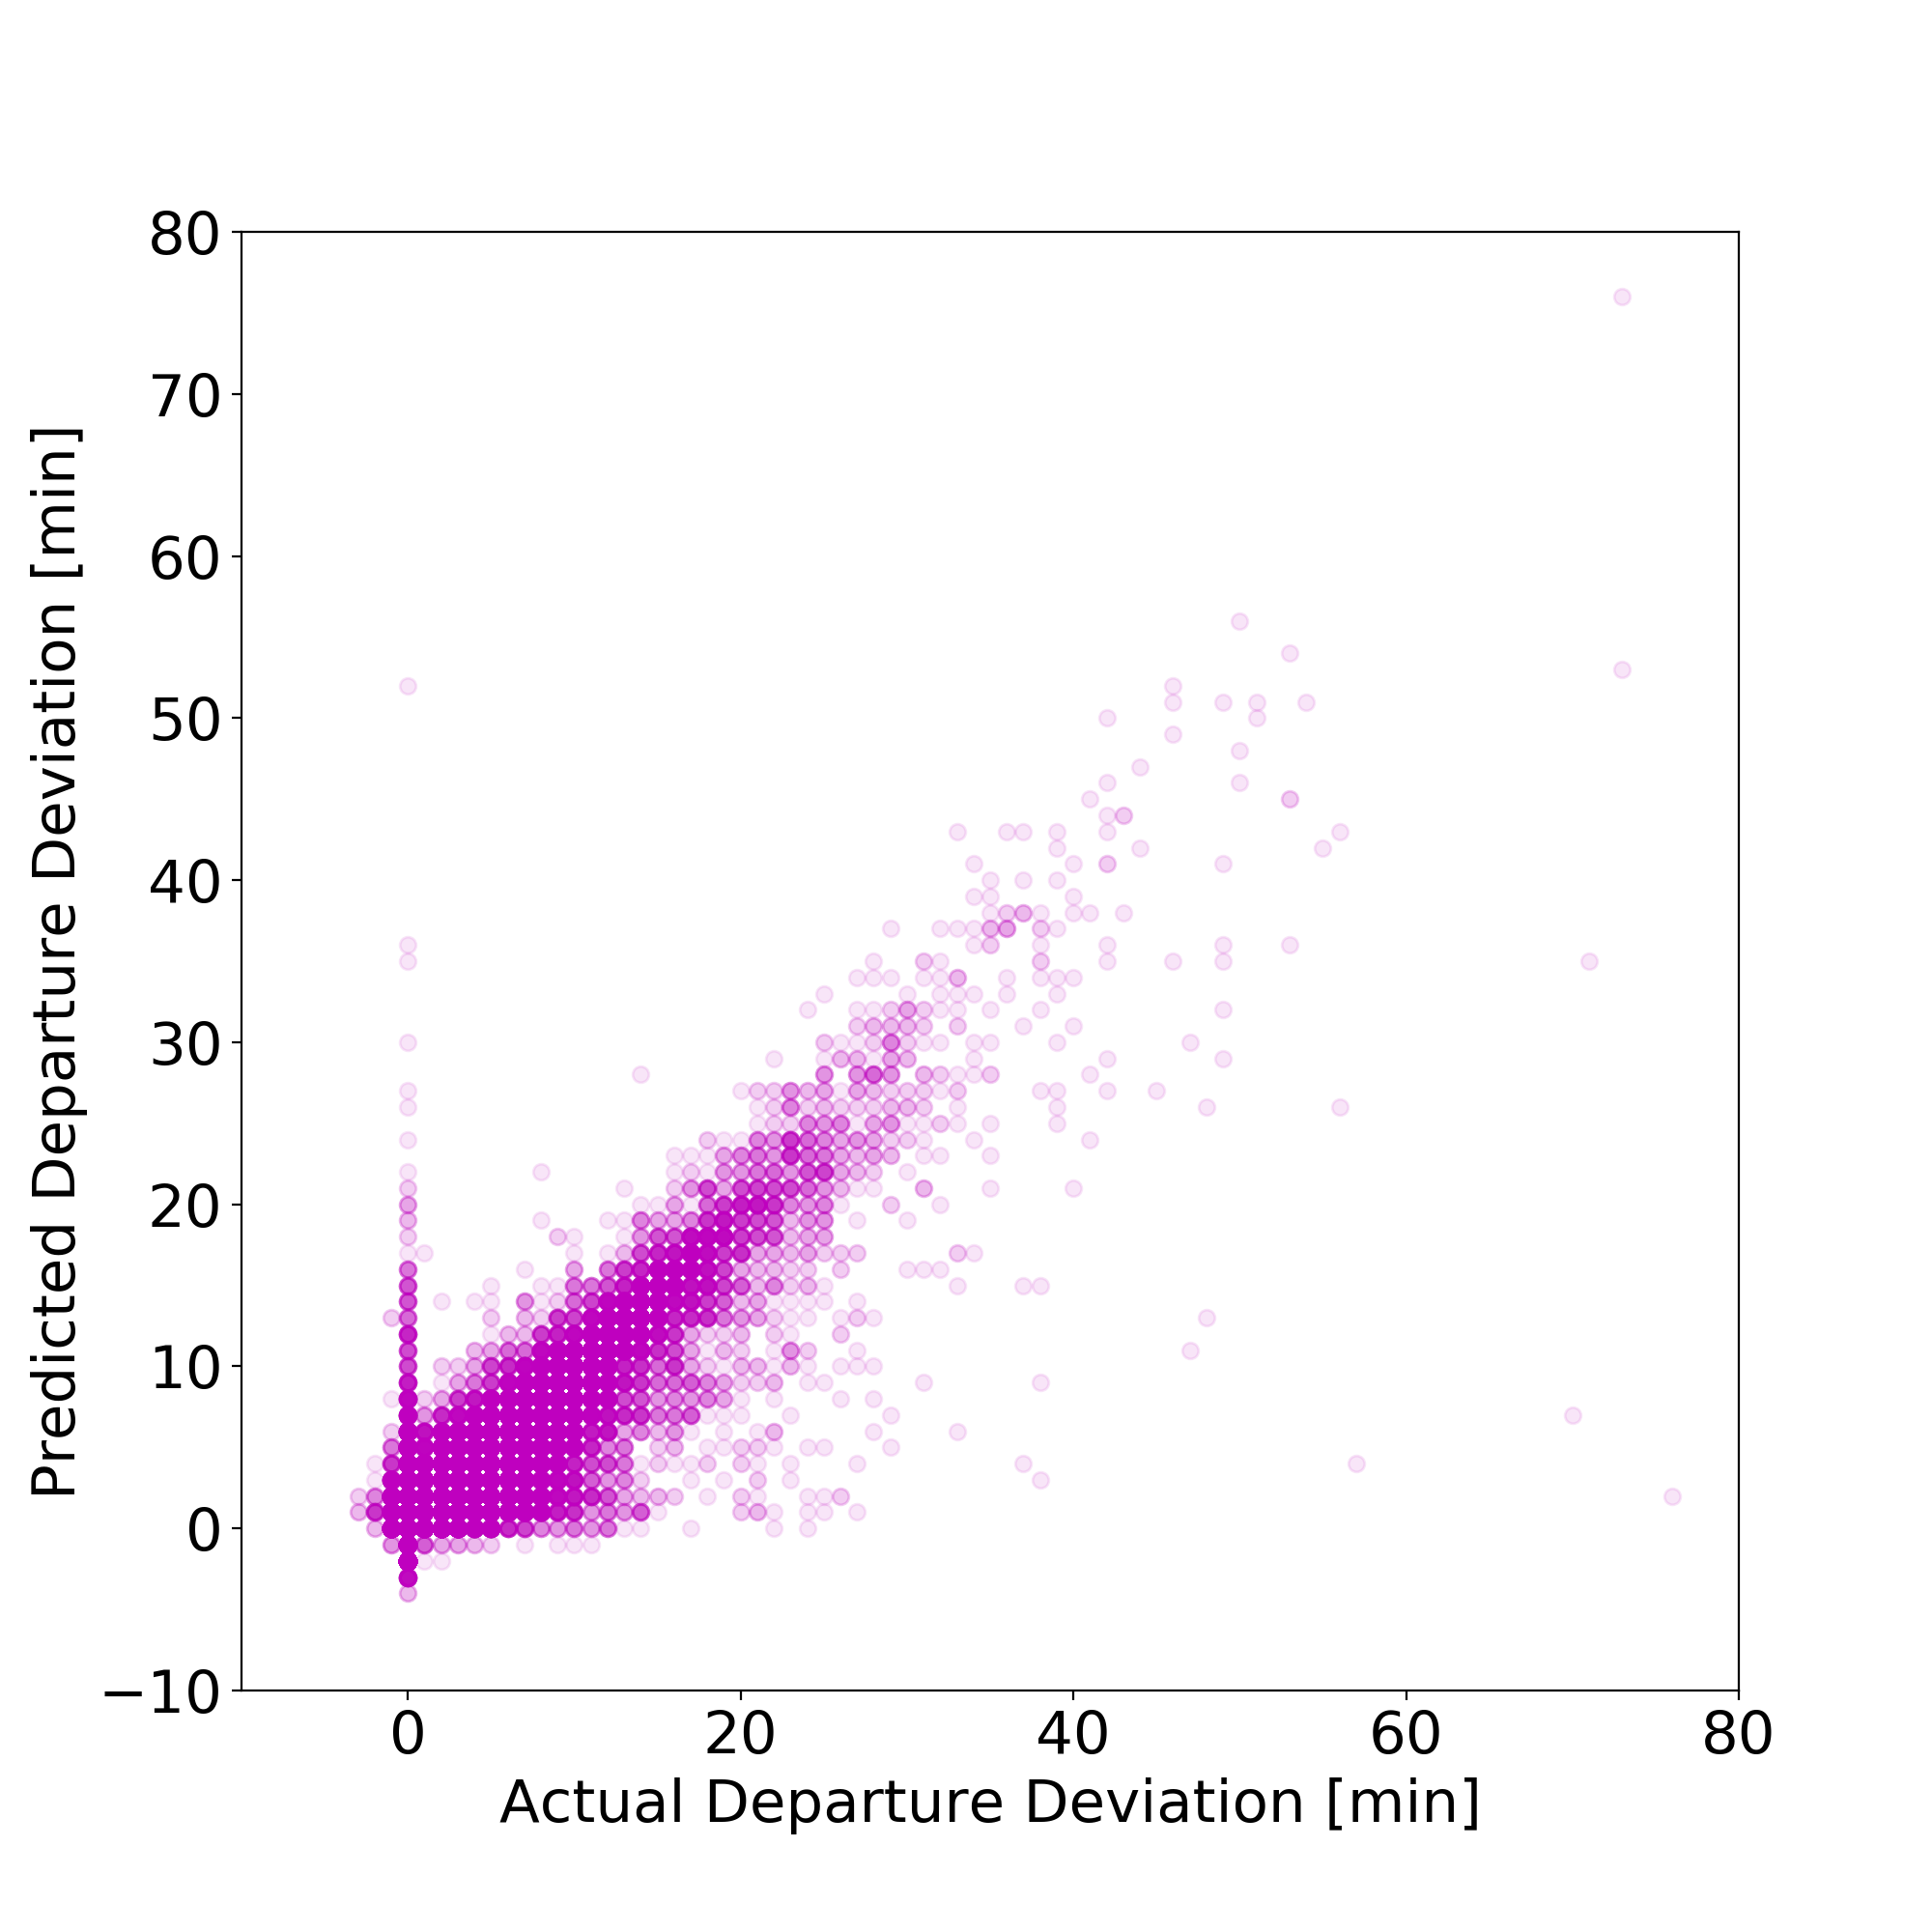
\includegraphics[width=0.5\textwidth]{Images/DNN_plot/1_step/1_step_depature_deviation.png}\label{fig:1_step_depature_deviation}}
     \subfloat[][XGBoost]{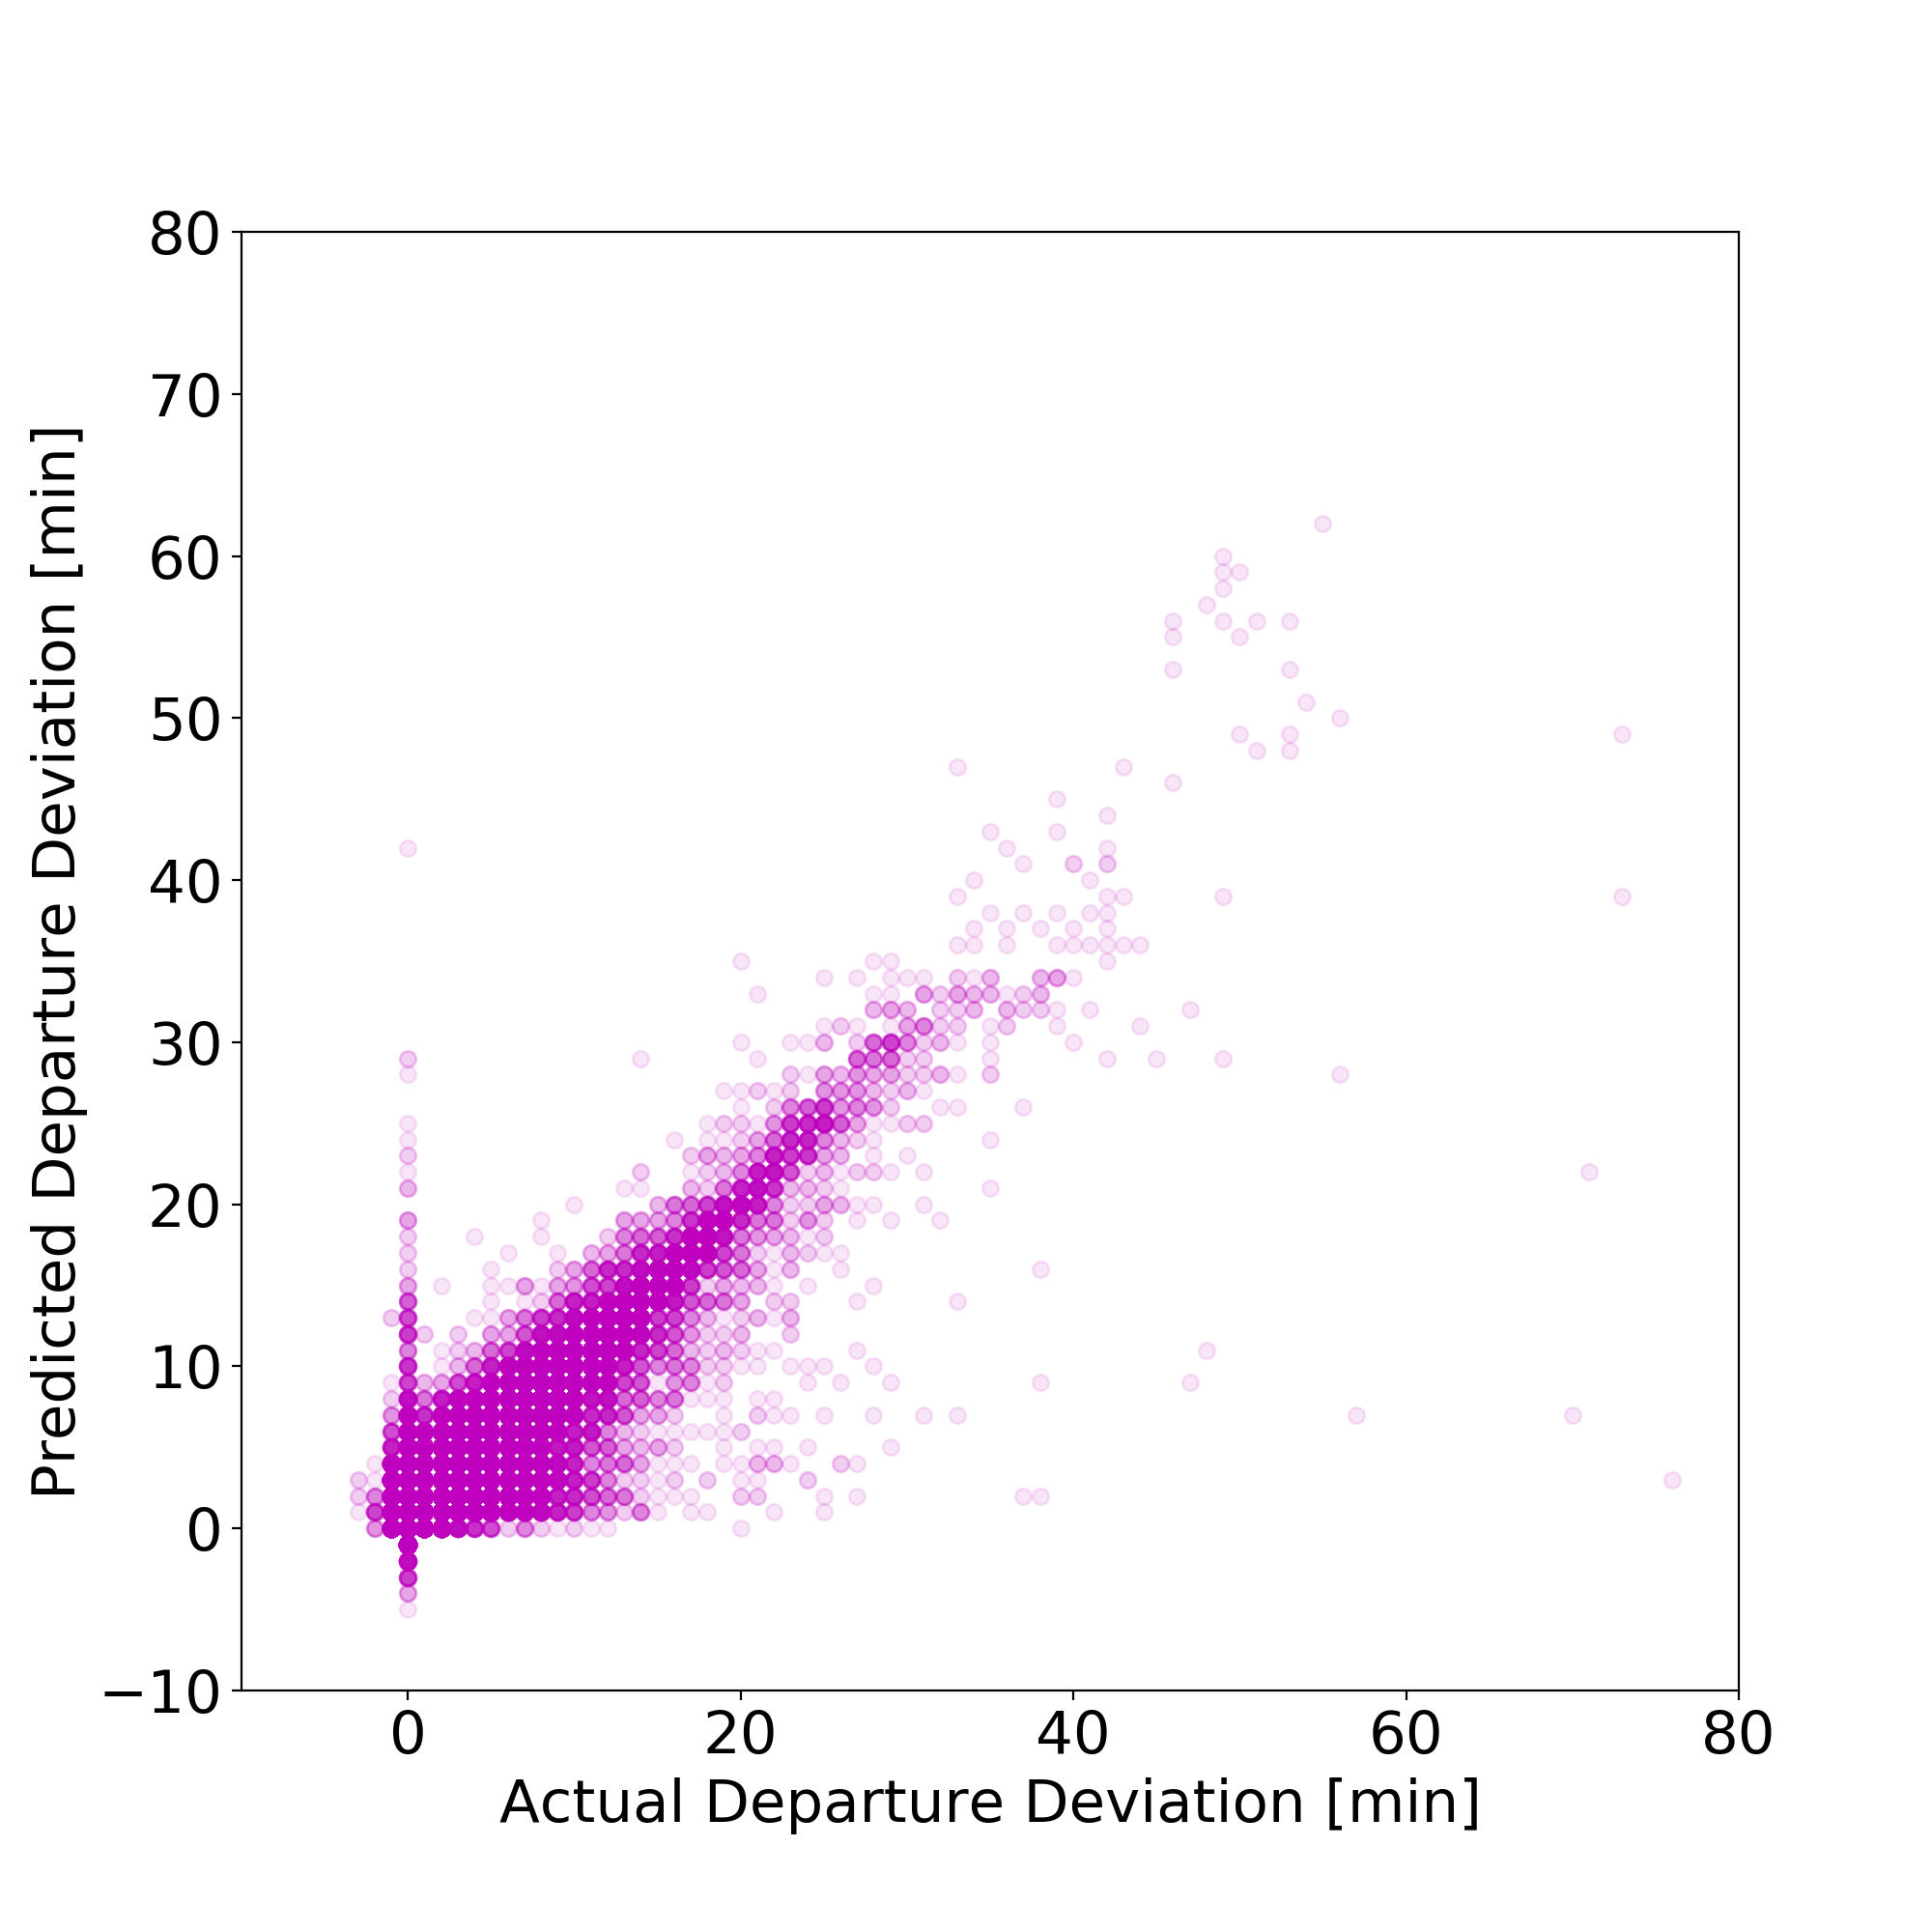
\includegraphics[width=0.5\textwidth]{Images/XGBoost_plot/1_step/1_step_depature_deviation.png}\label{fig:1_step_depature_deviation}}
    \caption{1-step predicted vs actual departure delay}
\end{figure}
\begin{figure}[H]
     \subfloat[][DNN]{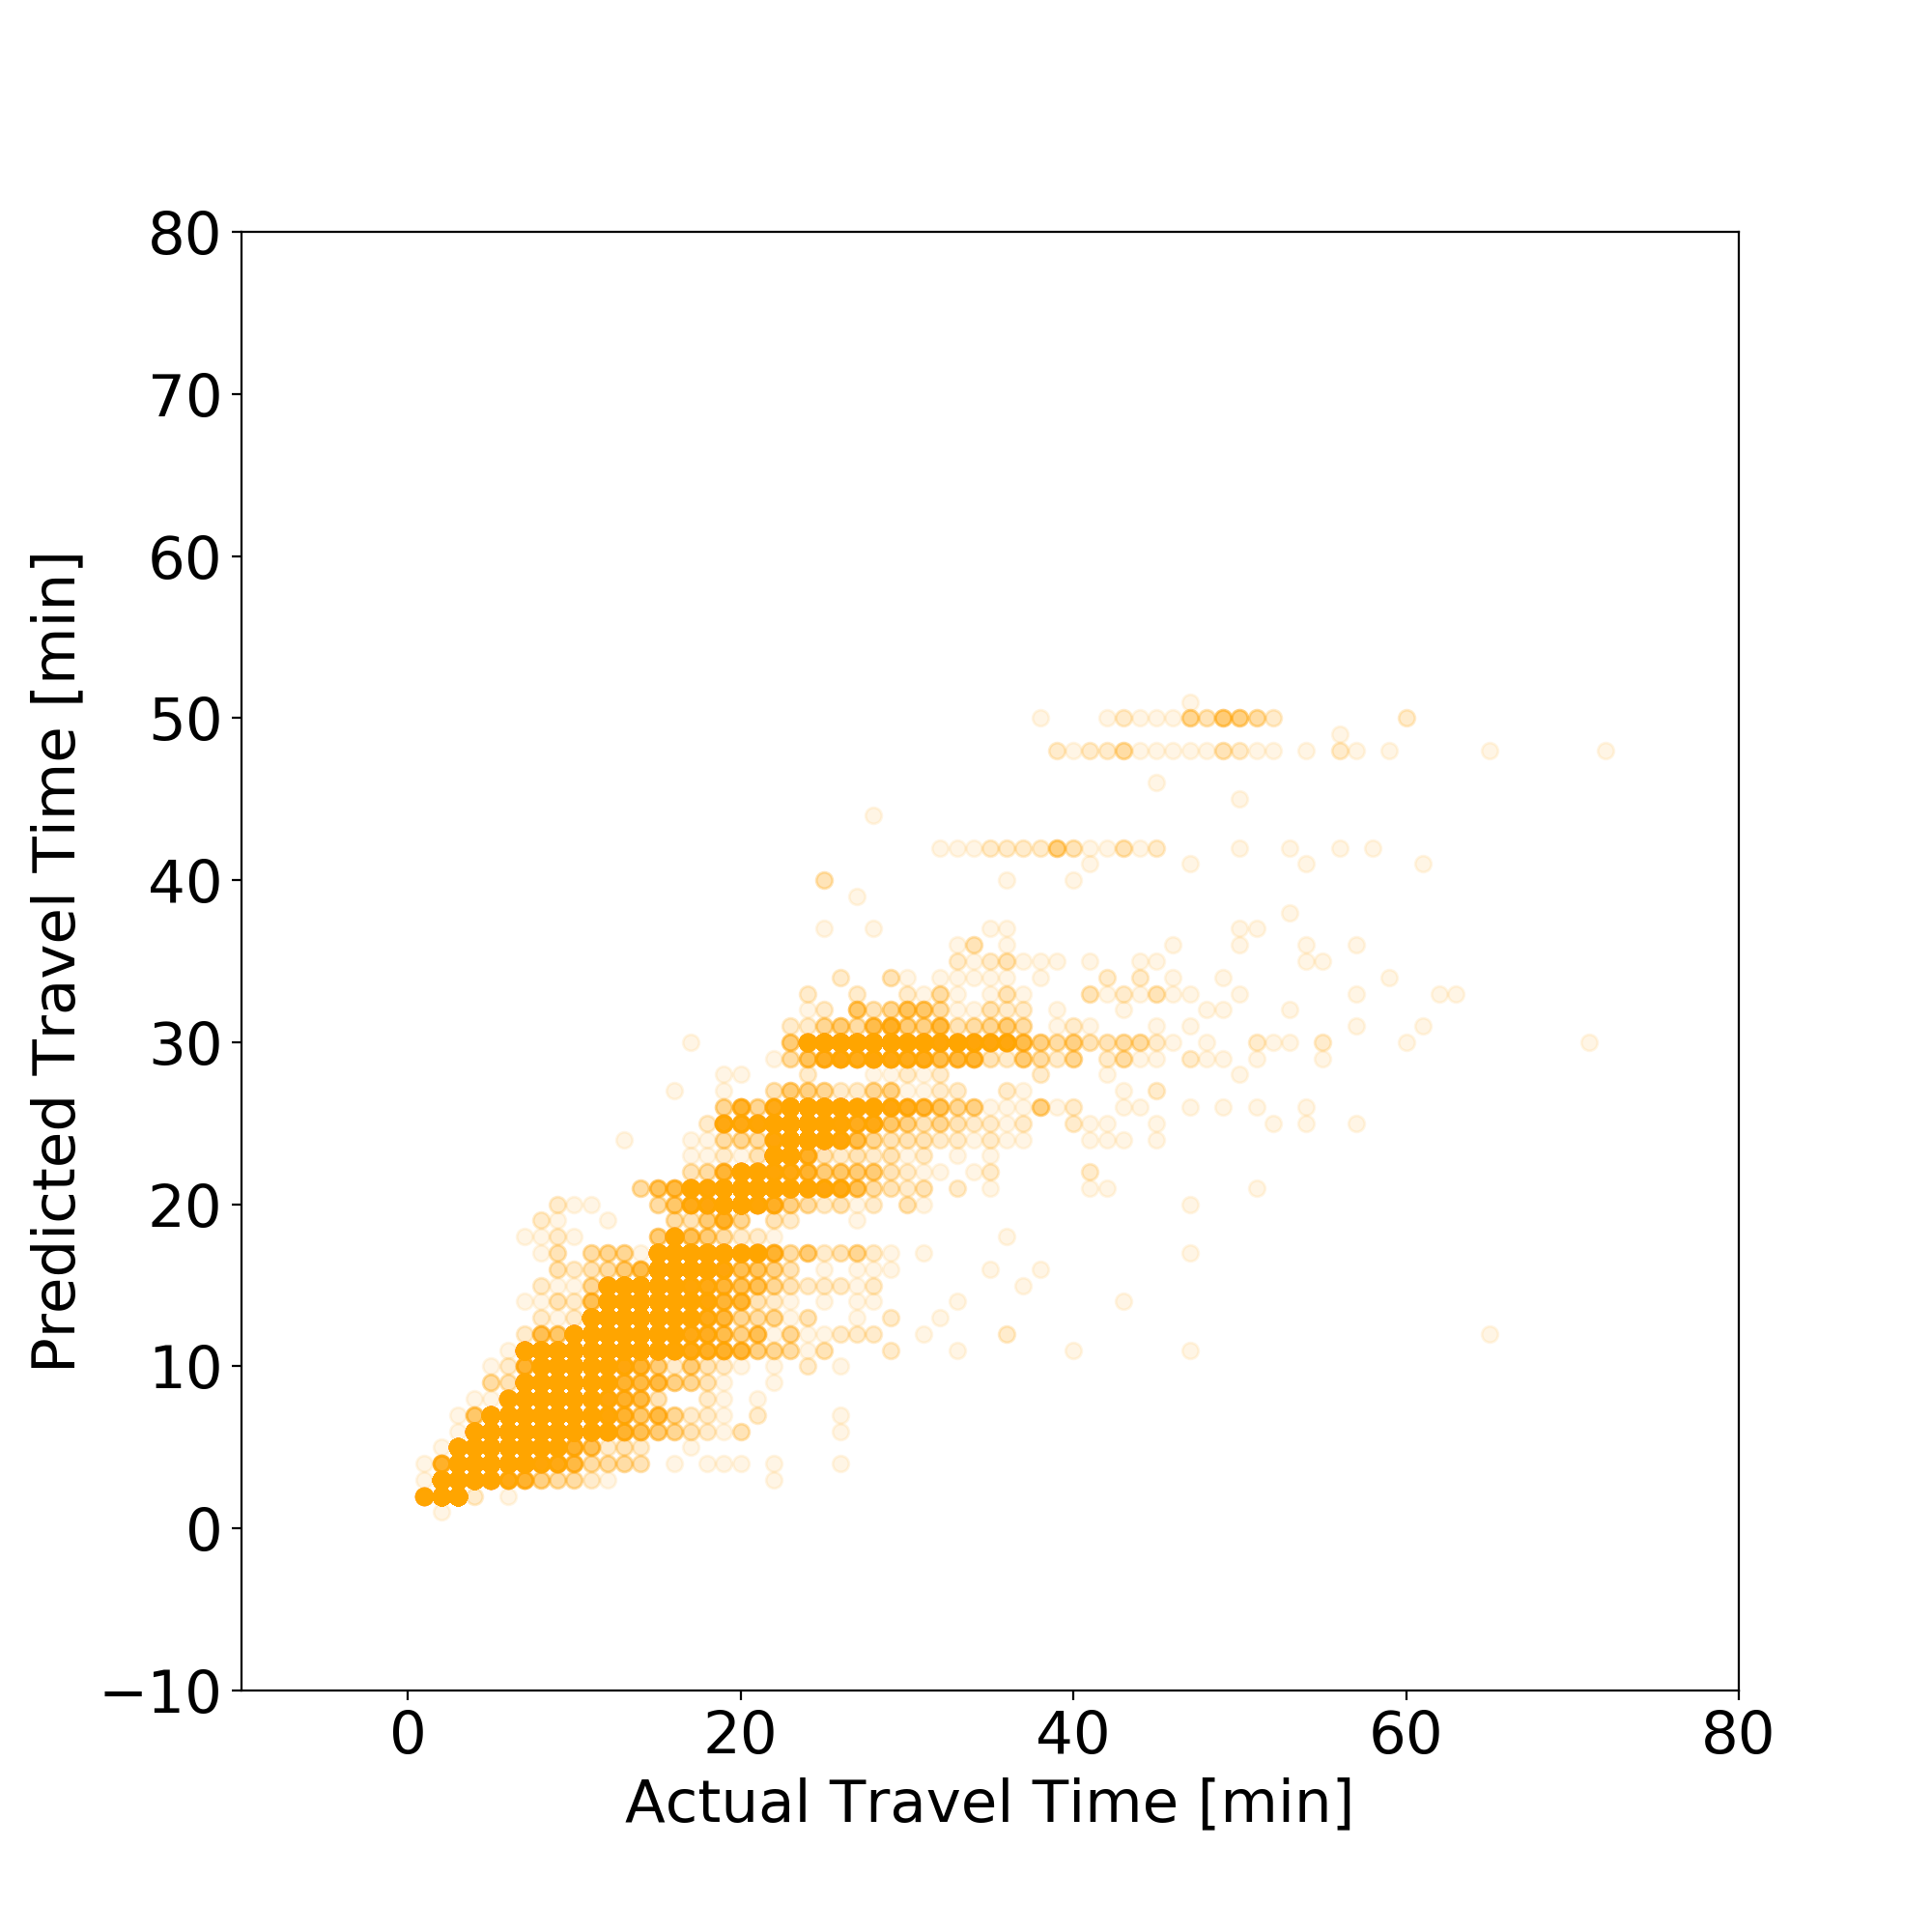
\includegraphics[width=0.5\textwidth]{Images/DNN_plot/1_step/1_step_travel_time.png}\label{fig:1_step_travel_time}}
     \subfloat[][XGBoost]{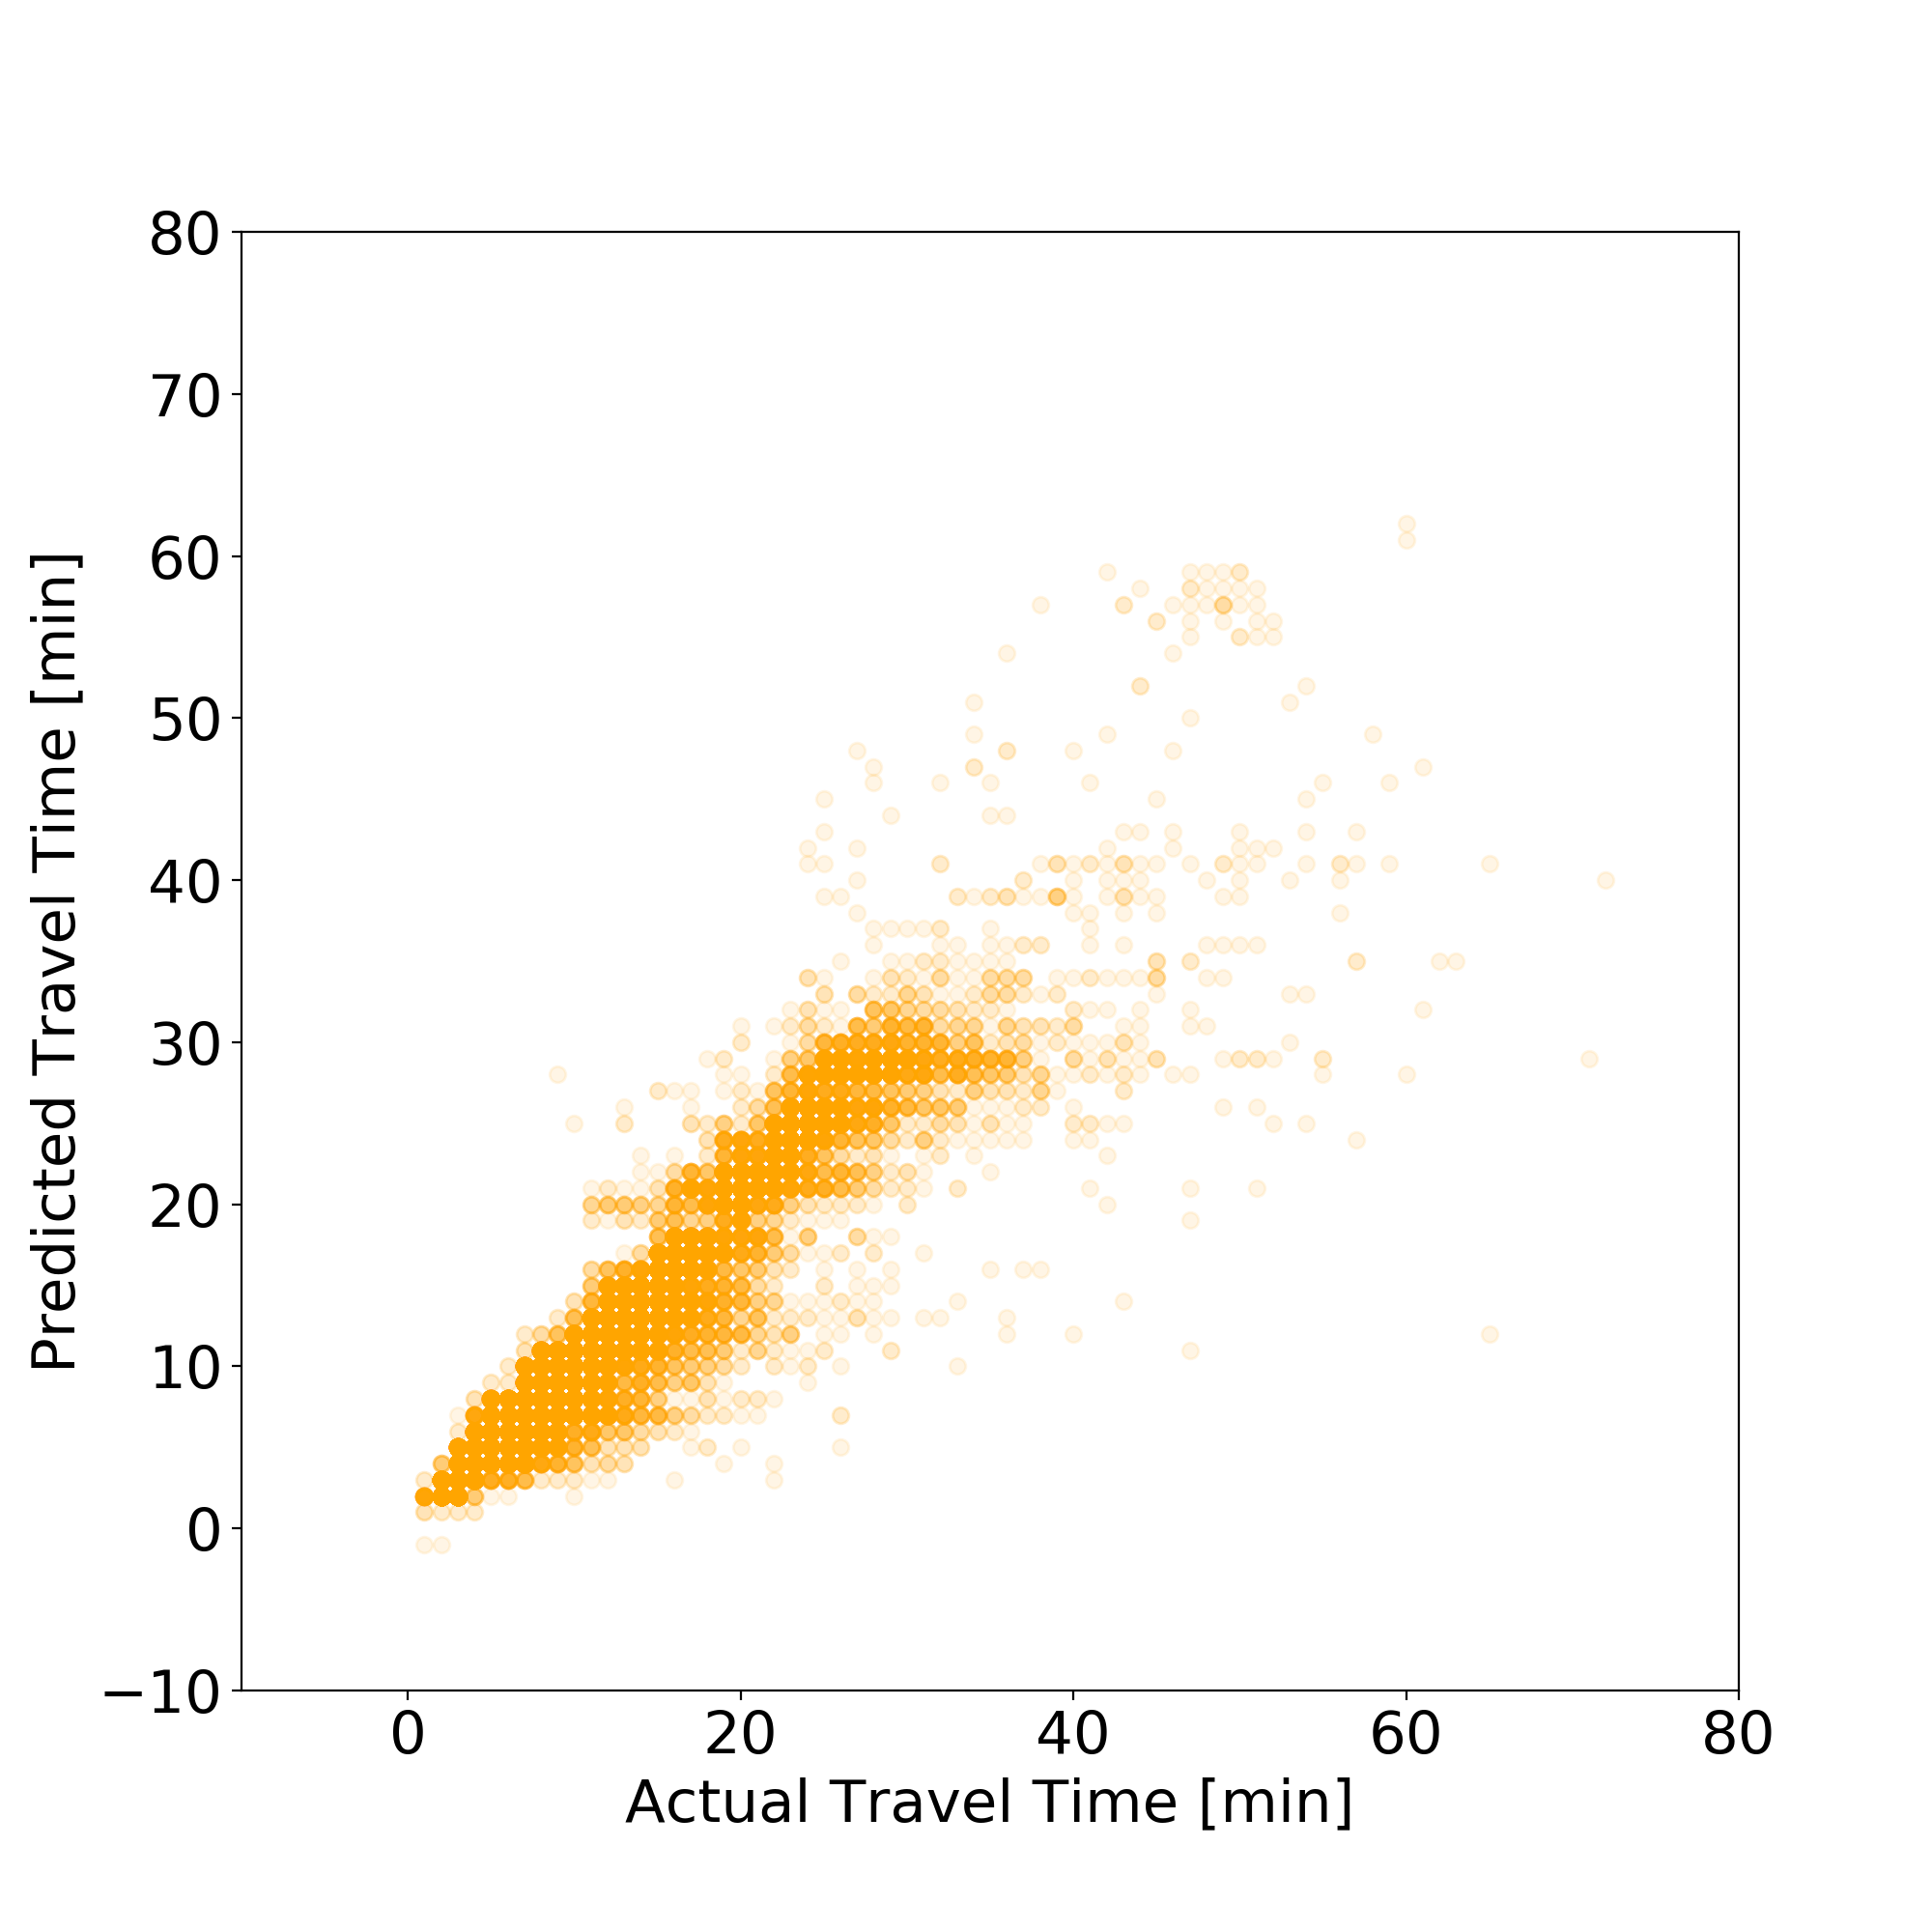
\includegraphics[width=0.5\textwidth]{Images/XGBoost_plot/1_step/1_step_travel_time.png}\label{fig:1_step_travel_time}}
    \caption{1-step predicted vs actual travel time}
\end{figure}
\begin{figure}[H]
     \subfloat[][DNN]{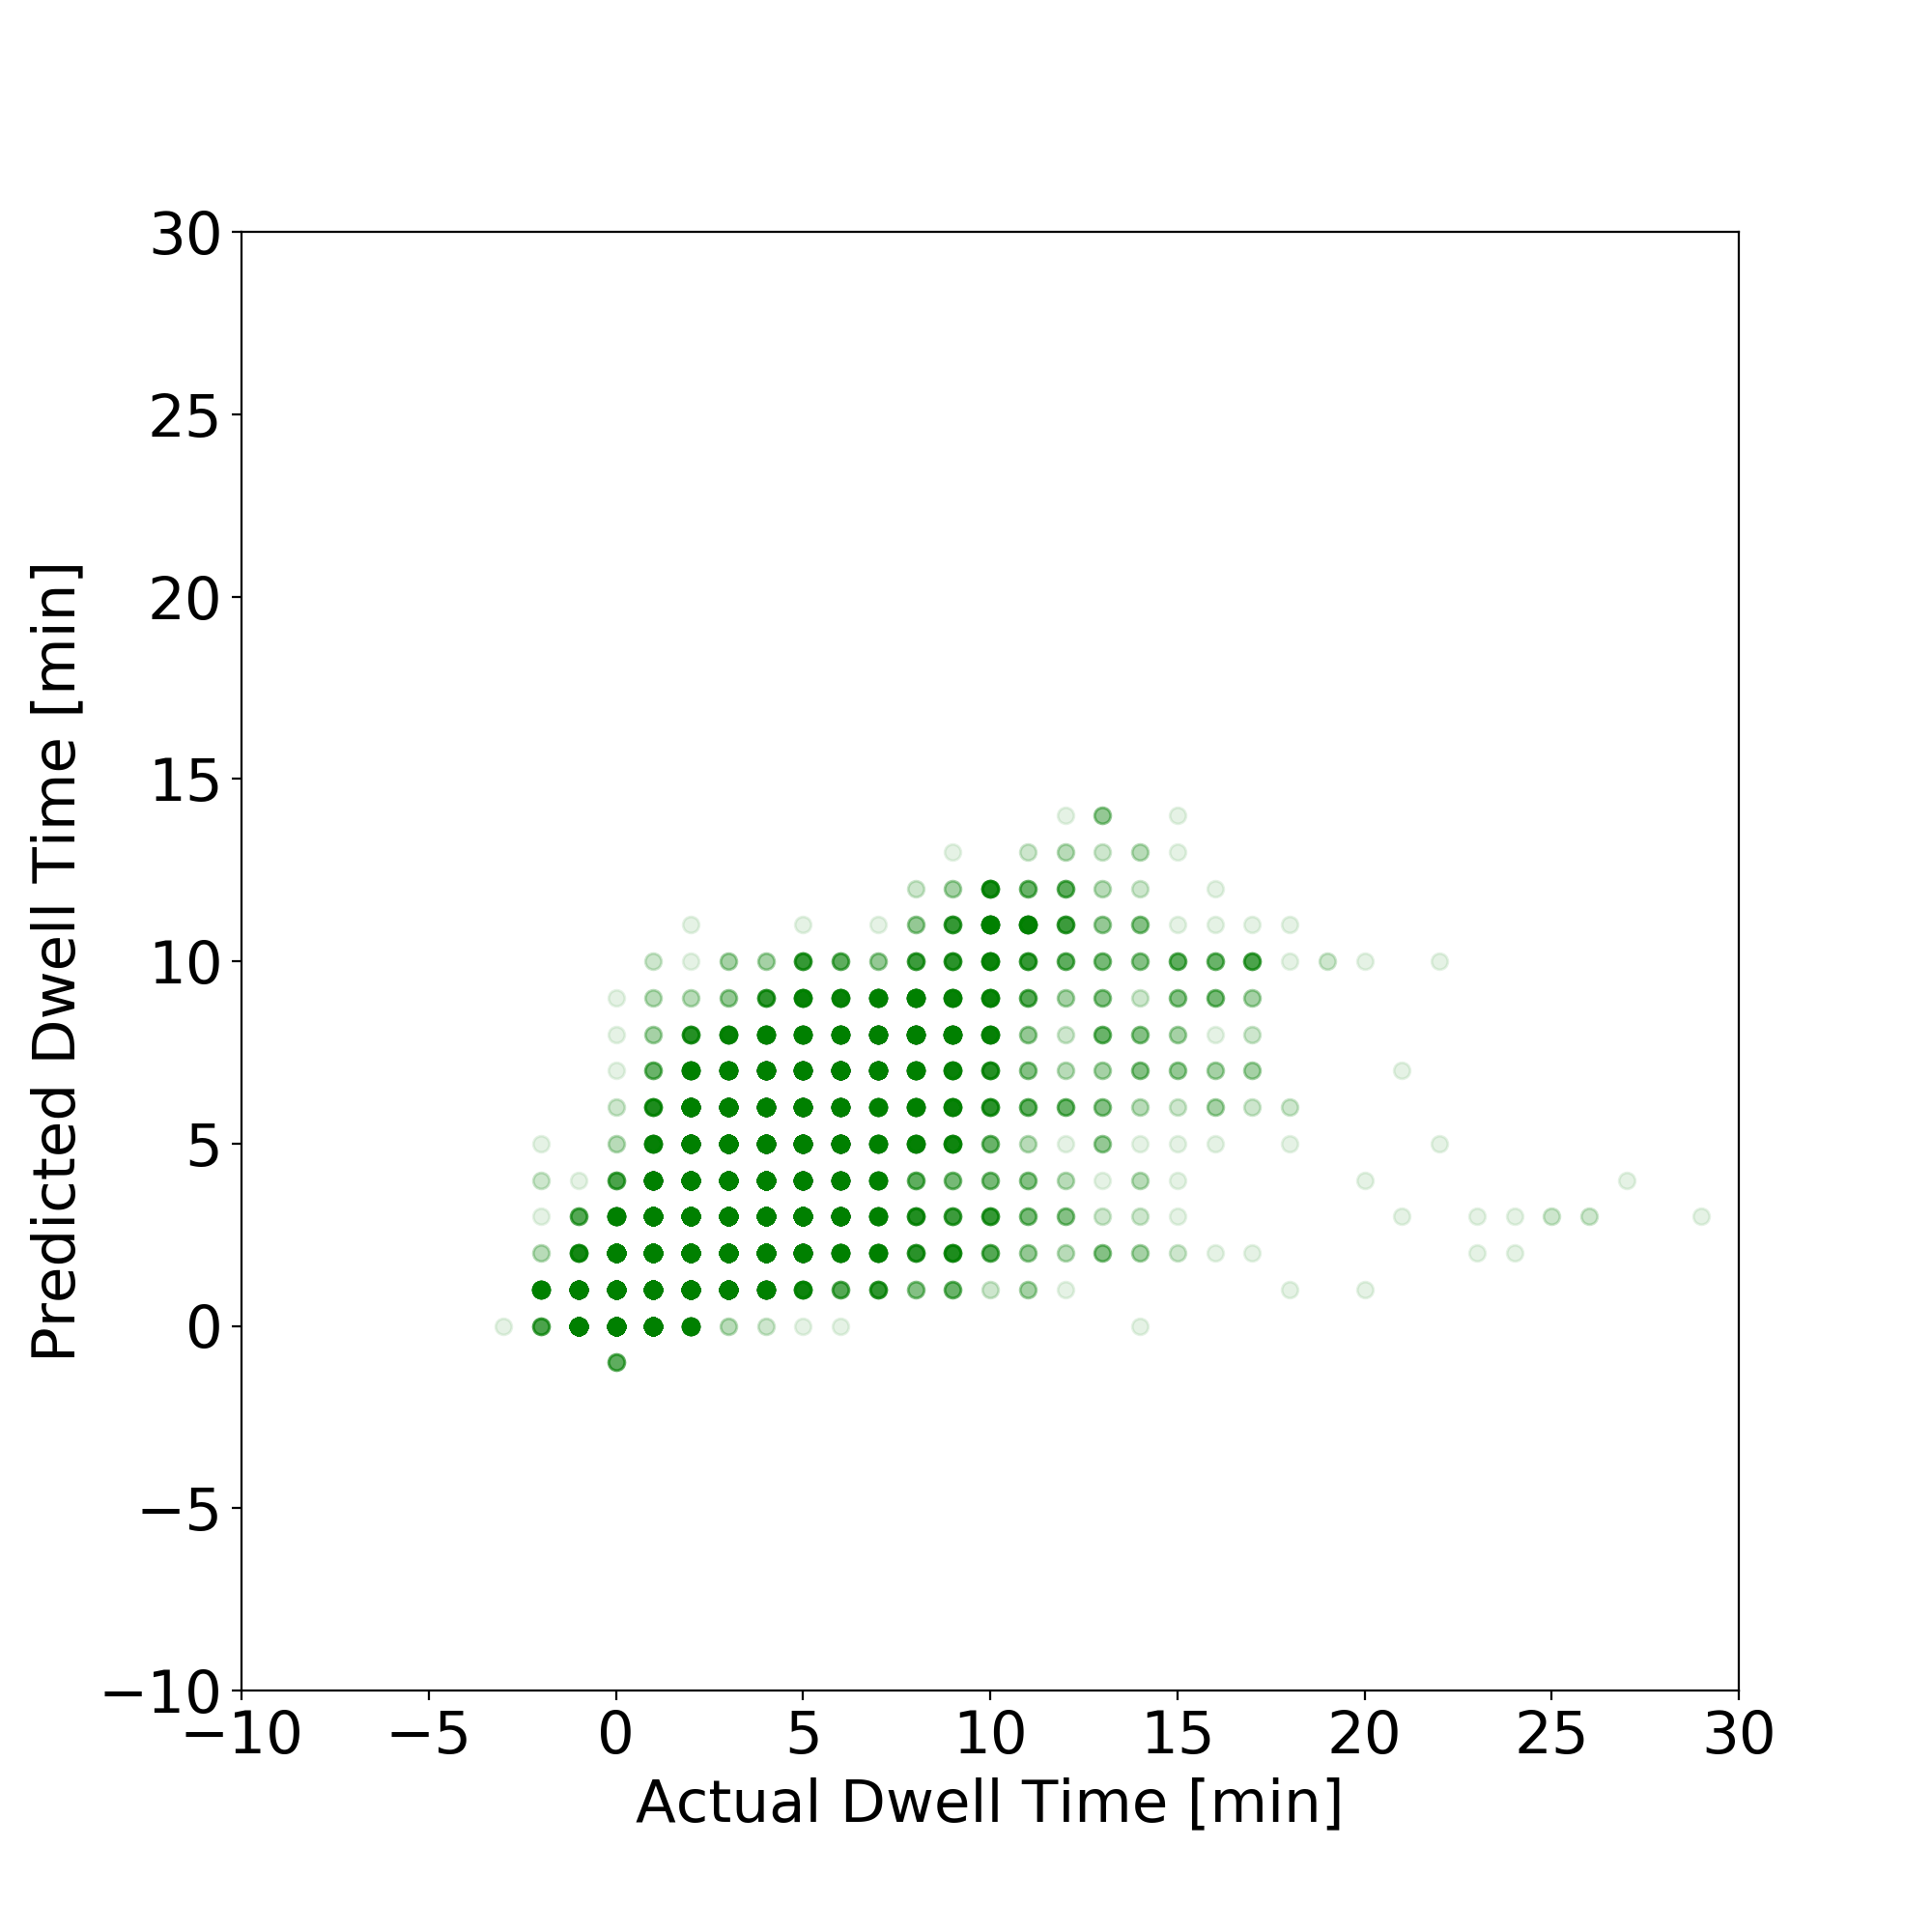
\includegraphics[width=0.5\textwidth]{Images/DNN_plot/1_step/1_step_dwell_time.png}\label{fig:1_step_dwell_time}}
     \subfloat[][XGBoost]{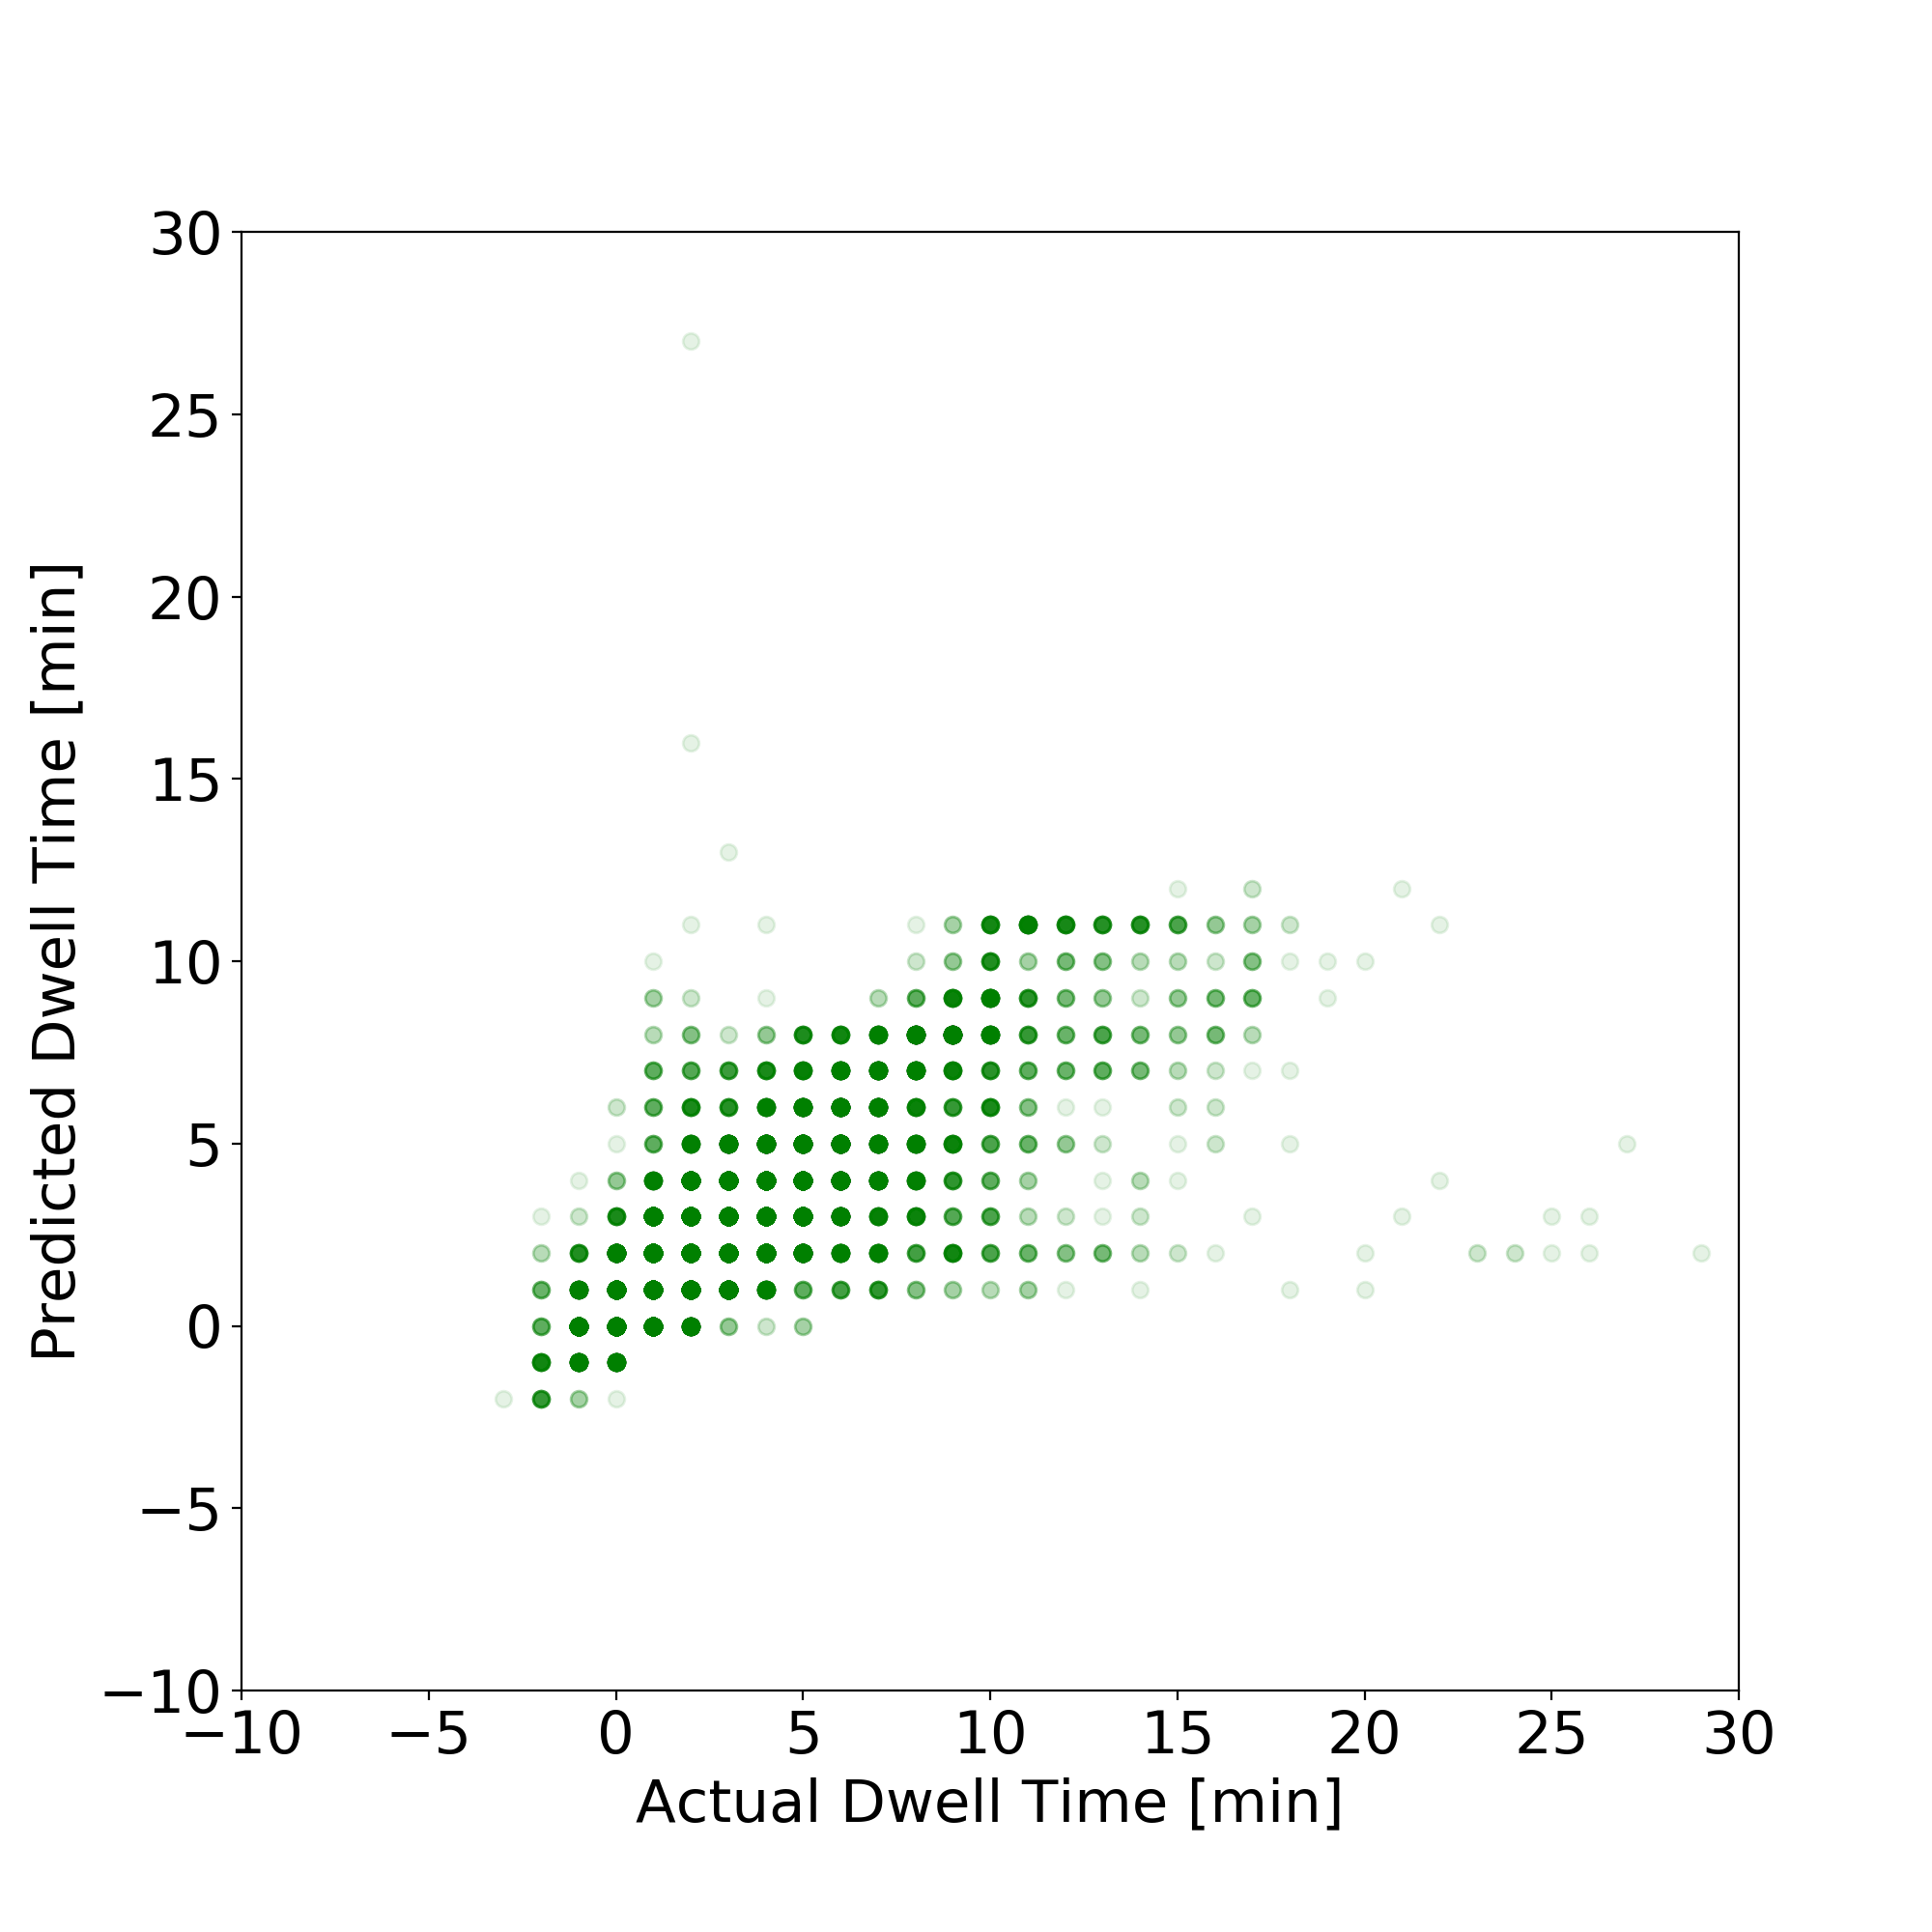
\includegraphics[width=0.5\textwidth]{Images/XGBoost_plot/1_step/1_step_dwell_time.png}\label{fig:1_step_dwell_time}}
     \caption{1-step predicted vs actual dwell time}
     \label{fig:1_step_dwell_time}
\end{figure}

\begin{table}[H]
\tbl{Model performance for arrival deviation forecasting}
{\begin{tabular}{lccccccccc} \toprule
  &  \multicolumn{4}{c}{DNN}  & \multicolumn{1}{c}{\quad} & \multicolumn{4}{c}{XGBoost} \\ \cmidrule{2-10}
 Step  &  RMSE  &  $r^2$  &  AADAE & MAAPE & \quad &  RMSE  &  $r^2$  &  AADAE & MAAPE \\ \midrule
1 & 2.03 & 0.83 & 1.10 & 1.11 & \quad & 1.91 & 0.85 & 1.03 & 1.08 \\ 
2 & 2.56 & 0.73 & 1.42 & 1.16 & \quad & 2.46 & 0.75 & 1.36 & 1.13 \\ 
3 & 2.76 & 0.66 & 1.58 & 1.17 & \quad & 2.62 & 0.69 & 1.41 & 1.17 \\ 
4 & 2.82 & 0.61 & 1.52 & 1.23 & \quad & 2.73 & 0.64 & 1.44 & 1.21 \\ 
5 & 2.81 & 0.57 & 1.39 & 1.28 & \quad & 2.67 & 0.61 & 1.34 & 1.26 \\ 
6 & 2.72 & 0.55 & 1.30 & 1.31 & \quad & 2.63 & 0.58 & 1.25 & 1.30 \\ 
7 & 2.73 & 0.49 & 1.22 & 1.34 & \quad & 2.59 & 0.54 & 1.21 & 1.33 \\ 
8 & 2.67 & 0.46 & 1.17 & 1.36 & \quad & 2.56 & 0.50 & 1.12 & 1.35 \\ 
9 & 2.56 & 0.45 & 1.09 & 1.38 & \quad & 2.54 & 0.46 & 1.05 & 1.38 \\ 
10 & 2.53 & 0.42 & 1.00 & 1.41 & \quad & 2.46 & 0.45 & 0.96 & 1.40 \\ 
\bottomrule
  &  \multicolumn{4}{c}{Multiple Linear Regression}  & \multicolumn{1}{c}{\quad} & \multicolumn{4}{c}{Decision Tree} \\ \cmidrule{2-10}
 Step  &  RMSE  &  $r^2$  &  AADAE & MAAPE & \quad &  RMSE  &  $r^2$  &  AADAE & MAAPE \\ \midrule
1 & 2.11 & 0.82 & 1.18 & 1.09 & \quad & 2.92 & 0.65 & 1.42 & 1.11 \\ 
2 & 3.14 & 0.59 & 1.89 & 1.12 & \quad & 3.68 & 0.44 & 1.90 & 1.18 \\ 
3 & 3.52 & 0.45 & 2.20 & 1.16 & \quad & 5.67 & -0.43 & 2.47 & 1.24 \\ 
4 & 3.64 & 0.36 & 2.27 & 1.21 & \quad & 4.33 & 0.09 & 2.13 & 1.28 \\ 
5 & 3.58 & 0.31 & 2.16 & 1.26 & \quad & 4.07 & 0.11 & 1.97 & 1.32 \\ 
6 & 3.46 & 0.27 & 2.00 & 1.29 & \quad & 4.12 & -0.04 & 1.86 & 1.35 \\ 
7 & 3.34 & 0.23 & 1.82 & 1.32 & \quad & 3.98 & -0.09 & 1.68 & 1.38 \\ 
8 & 3.22 & 0.21 & 1.65 & 1.34 & \quad & 4.04 & -0.24 & 1.63 & 1.40 \\ 
9 & 3.07 & 0.20 & 1.49 & 1.37 & \quad & 3.79 & -0.22 & 1.49 & 1.42 \\ 
10 & 2.97 & 0.20 & 1.36 & 1.40 & \quad & 3.81 & -0.32 & 1.40 & 1.44 \\ 
\bottomrule
\end{tabular}}
\label{table:ArrivalDeviationPrediction}
\end{table}

\begin{table}[H]
\tbl{Model performance for departure deviation forecasting}
{\begin{tabular}{lccccccccc} \toprule
  &  \multicolumn{4}{c}{DNN}  & \multicolumn{1}{c}{\quad} & \multicolumn{4}{c}{XGBoost} \\ \cmidrule{2-10}
 Step  &  RMSE  &  $r^2$  &  ADDAE & MAAPE & \quad &  RMSE  &  $r^2$  &  ADDAE & MAAPE \\ \midrule
1 & 2.05 & 0.80 & 1.15 & 1.11 & \quad & 1.99 & 0.81 & 1.08 & 1.11 \\
2 & 2.66 & 0.65 & 1.48 & 1.18 & \quad & 2.23 & 0.75 & 1.21 & 1.18 \\
3 & 2.82 & 0.58 & 1.56 & 1.25 & \quad & 2.39 & 0.70 & 1.28 & 1.24 \\
4 & 2.75 & 0.56 & 1.46 & 1.29 & \quad & 2.40 & 0.67 & 1.26 & 1.29 \\
5 & 2.68 & 0.54 & 1.30 & 1.32 & \quad & 2.38 & 0.64 & 1.19 & 1.33 \\
6 & 2.57 & 0.53 & 1.20 & 1.35 & \quad & 2.30 & 0.62 & 1.09 & 1.35 \\
7 & 2.51 & 0.50 & 1.12 & 1.37 & \quad & 2.29 & 0.58 & 1.04 & 1.38 \\
8 & 2.43 & 0.48 & 1.03 & 1.40 & \quad & 2.33 & 0.52 & 1.03 & 1.40 \\
9 & 2.32 & 0.46 & 0.96 & 1.41 & \quad & 2.33 & 0.46 & 0.94 & 1.42 \\
10 & 2.21 & 0.45 & 0.85 & 1.44 & \quad & 2.09 & 0.51 & 0.82 & 1.44 \\
\bottomrule
  &  \multicolumn{4}{c}{Multiple Linear Regression}  & \multicolumn{1}{c}{\quad} & \multicolumn{4}{c}{Decision Tree} \\ \cmidrule{2-10}
 Step  &  RMSE  &  $r^2$  &  ADDAE & MAAPE & \quad &  RMSE  &  $r^2$  &  ADDAE & MAAPE \\ \midrule
1 & 2.68 & 0.66 & 1.55 & 1.12 & \quad & 2.65 & 0.66 & 1.30 & 1.13 \\ 
2 & 3.30 & 0.46 & 2.09 & 1.21 & \quad & 3.28 & 0.47 & 1.72 & 1.22 \\ 
3 & 3.48 & 0.36 & 2.23 & 1.27 & \quad & 3.83 & 0.22 & 1.86 & 1.27 \\ 
4 & 3.45 & 0.32 & 2.16 & 1.31 & \quad & 3.91 & 0.12 & 1.84 & 1.32 \\ 
5 & 3.35 & 0.28 & 2.02 & 1.35 & \quad & 3.70 & 0.13 & 1.62 & 1.35 \\ 
6 & 3.23 & 0.25 & 1.85 & 1.38 & \quad & 3.75 & -0.00 & 1.60 & 1.38 \\ 
7 & 3.09 & 0.25 & 1.66 & 1.40 & \quad & 4.15 & -0.36 & 1.58 & 1.40 \\ 
8 & 2.94 & 0.23 & 1.50 & 1.42 & \quad & 3.51 & -0.09 & 1.40 & 1.42 \\ 
9 & 2.75 & 0.24 & 1.34 & 1.43 & \quad & 3.28 & -0.07 & 1.24 & 1.44 \\ 
10 & 2.61 & 0.23 & 1.23 & 1.45 & \quad & 3.30 & -0.22 & 1.16 & 1.45 \\ 
\bottomrule
\end{tabular}}
\label{table:DepartureDeviationPrediction}
\end{table}

\begin{table}[H]
\tbl{Model performance for travel time forecasting}
{\begin{tabular}{lccccccccc} \toprule
  &  \multicolumn{4}{c}{DNN}  & \multicolumn{1}{c}{\quad} & \multicolumn{4}{c}{XGBoost} \\ \cmidrule{2-10}
 Step  &  RMSE  &  $r^2$  &  ATTAE & MAAPE & \quad &  RMSE  &  $r^2$  &  ATTAE & MAAPE \\ \midrule
1 & 1.77 & 0.93 & 0.82 & 1.31 & \quad & 1.74 & 0.93 & 0.79 & 1.31 \\
2 & 1.74 & 0.93 & 0.78 & 1.33 & \quad & 1.73 & 0.94 & 0.72 & 1.33 \\
3 & 1.62 & 0.93 & 0.76 & 1.36 & \quad & 1.57 & 0.94 & 0.62 & 1.36 \\
4 & 1.47 & 0.94 & 0.60 & 1.38 & \quad & 1.46 & 0.95 & 0.55 & 1.38 \\
5 & 1.38 & 0.95 & 0.50 & 1.40 & \quad & 1.35 & 0.95 & 0.45 & 1.40 \\
6 & 1.22 & 0.95 & 0.41 & 1.42 & \quad & 1.19 & 0.95 & 0.37 & 1.42 \\
7 & 1.21 & 0.94 & 0.38 & 1.43 & \quad & 1.14 & 0.95 & 0.33 & 1.43 \\
8 & 1.16 & 0.94 & 0.34 & 1.45 & \quad & 1.11 & 0.95 & 0.32 & 1.45 \\
9 & 1.05 & 0.95 & 0.29 & 1.46 & \quad & 1.04 & 0.95 & 0.28 & 1.46 \\
10 & 1.18 & 0.94 & 0.28 & 1.47 & \quad & 1.14 & 0.94 & 0.28 & 1.47 \\
\bottomrule
  &  \multicolumn{4}{c}{Multiple Linear Regression}  & \multicolumn{1}{c}{\quad} & \multicolumn{4}{c}{Decision Tree} \\ \cmidrule{2-10}
 Step  &  RMSE  &  $r^2$  &  ATTAE & MAAPE & \quad &  RMSE  &  $r^2$  &  ATTAE & MAAPE \\ \midrule
1 & 1.78 & 0.93 & 0.83 & 1.31 & \quad & 2.90 & 0.80 & 1.22 & 1.31 \\
2 & 1.71 & 0.94 & 0.75 & 1.33 & \quad & 2.75 & 0.84 & 1.13 & 1.33 \\
3 & 1.55 & 0.94 & 0.64 & 1.36 & \quad & 2.63 & 0.83 & 1.00 & 1.36 \\
4 & 1.46 & 0.95 & 0.57 & 1.38 & \quad & 2.25 & 0.87 & 0.87 & 1.38 \\
5 & 1.35 & 0.95 & 0.47 & 1.40 & \quad & 2.09 & 0.88 & 0.83 & 1.40 \\
6 & 1.18 & 0.95 & 0.38 & 1.42 & \quad & 1.90 & 0.87 & 0.60 & 1.42 \\
7 & 1.13 & 0.95 & 0.33 & 1.44 & \quad & 1.65 & 0.89 & 0.53 & 1.43 \\
8 & 1.10 & 0.95 & 0.32 & 1.45 & \quad & 2.15 & 0.81 & 0.62 & 1.45 \\
9 & 1.02 & 0.95 & 0.28 & 1.46 & \quad & 1.59 & 0.88 & 0.48 & 1.46 \\
10 & 1.11 & 0.95 & 0.27 & 1.47 & \quad & 1.68 & 0.88 & 0.45 & 1.47 \\
\bottomrule
\end{tabular}}
\label{table:TravelTimePrediction}
\end{table}

\begin{table}[H]
\tbl{Model performance for dwell time forecasting}
{\begin{tabular}{lccccccccc} \toprule
  &  \multicolumn{4}{c}{DNN}  & \multicolumn{1}{c}{\quad} &  \multicolumn{4}{c}{XGBoost} \\ \cmidrule{2-10}
 Step  &  RMSE  &  $r^2$  &  ADTAE & MAAPE & \quad &  RMSE  &  $r^2$  &  ADTAE & MAAPE \\ \midrule
1 & 1.23 & 0.54 & 0.67 & 0.81 & \quad & 1.08 & 0.65 & 0.52 & 0.82 \\
2 & 1.32 & 0.47 & 0.69 & 0.88 & \quad & 1.11 & 0.63 & 0.53 & 0.82 \\
3 & 1.12 & 0.61 & 0.55 & 0.89 & \quad & 1.08 & 0.64 & 0.50 & 0.89 \\
4 & 1.11 & 0.60 & 0.50 & 0.96 & \quad & 1.04 & 0.64 & 0.44 & 0.99 \\
5 & 0.99 & 0.67 & 0.42 & 1.01 & \quad & 0.94 & 0.70 & 0.39 & 1.04 \\
6 & 1.00 & 0.66 & 0.40 & 1.08 & \quad & 0.92 & 0.71 & 0.36 & 1.10 \\
7 & 0.91 & 0.71 & 0.35 & 1.14 & \quad & 0.96 & 0.68 & 0.38 & 1.17 \\
8 & 1.09 & 0.56 & 0.46 & 1.22 & \quad & 0.79 & 0.77 & 0.29 & 1.19 \\
9 & 0.85 & 0.72 & 0.29 & 1.22 & \quad & 0.72 & 0.80 & 0.25 & 1.23 \\
10 & 0.80 & 0.74 & 0.25 & 1.24 & \quad & 0.80 & 0.74 & 0.24 & 1.26 \\
\bottomrule
  &  \multicolumn{4}{c}{Multiple Linear Regression}  & \multicolumn{1}{c}{\quad} &  \multicolumn{4}{c}{Decision Tree} \\ \cmidrule{2-10}
 Step  &  RMSE  &  $r^2$  &  ADTAE & MAAPE & \quad &  RMSE  &  $r^2$  &  ADTAE & MAAPE \\ \midrule
1 & 1.43 & 0.38 & 0.77 & 0.85 & \quad & 1.56 & 0.26 & 0.70 & 0.87  \\
2 & 1.41 & 0.39 & 0.76 & 0.84 & \quad & 1.97 & -0.18 & 0.93 & 0.90 \\
3 & 1.35 & 0.43 & 0.69 & 0.92 & \quad & 1.62 & 0.18 & 0.64 & 0.94  \\
4 & 1.27 & 0.47 & 0.59 & 0.98 & \quad & 1.47 & 0.29 & 0.61 & 1.03  \\
5 & 1.22 & 0.50 & 0.52 & 1.04 & \quad & 1.55 & 0.18 & 0.53 & 1.09  \\
6 & 1.18 & 0.53 & 0.47 & 1.10 & \quad & 1.55 & 0.17 & 0.50 & 1.16  \\
7 & 1.15 & 0.54 & 0.44 & 1.16 & \quad & 1.20 & 0.49 & 0.41 & 1.19  \\
8 & 1.06 & 0.59 & 0.40 & 1.21 & \quad & 1.29 & 0.38 & 0.42 & 1.24  \\
9 & 1.00 & 0.61 & 0.35 & 1.25 & \quad & 1.02 & 0.59 & 0.33 & 1.25  \\
10 & 0.99 & 0.59 & 0.34 & 1.29 & \quad & 1.14 & 0.47 & 0.36 & 1.29  \\
\bottomrule
\end{tabular}}
\label{table:DwellTimePrediction}
\end{table}
\begin{table}[H]
    \tbl{DNN and XGBoost model training times}
    {\begin{tabular}{ccc}\toprule
        Model & DNN Training Time (s) & XGBoost Training Time (s) \\\hline
         1-step & 56.62 & 79.13\\
         2-step & 57.95 & 79.21\\
         3-step & 56.46 & 83.29\\
         4-step & 54.47 & 80.57\\
         5-step & 58.48 & 80.78\\
         6-step & 59.11 & 80.14\\
         7-step & 58.94 & 84.89\\
         8-step & 60.16 & 78.81\\
         9-step & 62.83 & 78.28\\
         10-step & 64.49 & 79.25\\
    \bottomrule
    \end{tabular}}
    \label{tab:XGBTrainTime}
\end{table}

\subsection{Performance Compared to Darwin}
 From Darwin's push port archive \citep{PET17}, we filtered out Darwin's forecasts from February to May of 2017 to match the train journeys in our case study and associated these forecasts with forecasts made by our DNN and XGBoost models. Unlike our model, Darwin did not forecast all train journeys within this time period, hence the number of analyzed journeys are significantly lower that that of section \ref{Subsection:ModelResults}. Furthermore, Darwin only predicts arrival times and departure times hence, only arrival and departure deviations will be computed from Darwin's forecasts and compared to that predicted by the DNN and XGBoost models.
\begin{table}[H]
\tbl{Model performance for arrival deviation forecasting vs Darwin}
{\begin{tabular}{lcccccccccccccc} \toprule
&  \multicolumn{4}{c}{DNN}  & \multicolumn{1}{c}{\quad} &  \multicolumn{4}{c}{XGBoost} & \multicolumn{1}{c}{\quad} &  \multicolumn{4}{c}{Darwin}\\ \cmidrule{2-15}
Step  &  RMSE  &  $r^2$  &  AADAE  & MAAPE & \quad &  RMSE  &  $r^2$  &  AADAE & MAAPE & \quad & RSME &  $r^2$  &  AADAE & MAAPE\\ \midrule
1 &  1.98 & 0.93 & 0.98 & 1.08 & \quad & 2.09 & 0.92 & 1.13 & 1.08 & \quad & 5.03 & 0.56 & 2.59 & 1.19\\
2 &  1.68 & 0.96 & 1.09 & 1.12 & \quad & 1.98 & 0.95 & 1.09 & 1.08 & \quad & 5.78 & 0.57 & 2.97 & 1.22\\
3 &  2.01 & 0.94 & 1.33 & 1.12 & \quad & 2.12 & 0.93 & 1.37 & 1.13 & \quad & 5.90 & 0.48 & 2.93 & 1.23\\
4 &  2.03 & 0.92 & 1.47 & 1.15 & \quad & 2.00 & 0.92 & 1.23 & 1.11 & \quad & 5.63 & 0.37 & 3.21 & 1.22\\
5 &  2.31 & 0.91 & 1.57 & 1.17 & \quad & 2.88 & 0.87 & 1.74 & 1.07 & \quad & 6.35 & 0.36 & 3.67 & 1.22\\
6 &  3.73 & 0.72 & 1.78 & 1.11 & \quad & 3.19 & 0.79 & 1.91 & 1.07 & \quad & 5.50 & 0.38 & 3.14 & 1.21\\
7 &  2.98 & 0.82 & 1.79 & 1.13 & \quad & 3.21 & 0.79 & 1.80 & 1.08 & \quad & 6.01 & 0.27 & 3.48 & 1.23\\
8 &  4.15 & 0.64 & 2.06 & 1.09 & \quad & 2.56 & 0.86 & 1.54 & 1.05 & \quad & 5.73 & 0.32 & 3.18 & 1.20\\
9 &  2.65 & 0.70 & 1.73 & 1.02 & \quad & 2.36 & 0.76 & 1.39 & 1.04 & \quad & 4.11 & 0.29 & 2.06 & 1.15\\
10 &  2.54 & 0.74 & 1.76 & 1.08 & \quad & 3.07 & 0.62 & 1.29 & 1.01 & \quad & 4.83 & 0.07 & 2.32 & 1.20\\
 \bottomrule
\end{tabular}}
\label{ArrivalDeviationPredictionVSDarwin}
\end{table}

\begin{table}[H]
\tbl{Model performance for departure deviation forecasting vs Darwin}
{\begin{tabular}{lcccccccccccccc} \toprule
&  \multicolumn{4}{c}{DNN}  & \multicolumn{1}{c}{\quad} &  \multicolumn{4}{c}{XGBoost} & \multicolumn{1}{c}{\quad} &  \multicolumn{4}{c}{Darwin}\\ \cmidrule{2-15}
Step  &  RMSE  &  $r^2$  &  AADAE  & MAAPE & \quad &  RMSE  &  $r^2$  &  AADAE & MAAPE & \quad & RSME &  $r^2$  &  AADAE & MAAPE\\ \midrule
1 &  1.82 & 0.94 & 0.94 & 0.92 & \quad & 1.96 & 0.93 & 1.06 & 0.91 & \quad & 5.77 & 0.42 & 3.41 & 1.11\\
2 &  3.75 & 0.82 & 1.76 & 1.03 & \quad & 5.34 & 0.64 & 1.63 & 1.03 & \quad & 6.27 & 0.50 & 3.42 & 1.17\\
3 &  3.02 & 0.86 & 1.38 & 0.98 & \quad & 6.80 & 0.28 & 2.20 & 1.01 & \quad & 6.40 & 0.36 & 3.63 & 1.19\\
4 &  2.65 & 0.86 & 1.59 & 1.11 & \quad & 2.36 & 0.89 & 1.32 & 1.09 & \quad & 5.89 & 0.31 & 3.42 & 1.24\\
5 &  3.71 & 0.78 & 2.27 & 1.13 & \quad & 3.65 & 0.79 & 2.15 & 1.14 & \quad & 6.98 & 0.23 & 4.43 & 1.24\\
6 &  3.76 & 0.68 & 1.80 & 1.07 & \quad & 3.50 & 0.72 & 1.86 & 1.11 & \quad & 5.94 & 0.19 & 3.66 & 1.25\\
7 &  3.52 & 0.75 & 2.05 & 1.12 & \quad & 3.38 & 0.77 & 1.70 & 1.12 & \quad & 6.53 & 0.14 & 4.11 & 1.25\\
8 &  4.51 & 0.57 & 2.18 & 1.13 & \quad & 3.27 & 0.77 & 1.76 & 1.13 & \quad & 6.07 & 0.22 & 3.33 & 1.28\\
9 &  3.59 & 0.46 & 2.08 & 1.14 & \quad & 3.41 & 0.52 & 1.82 & 1.11 & \quad & 4.37 & 0.21 & 2.20 & 1.22\\
10 &  2.72 & 0.69 & 1.64 & 0.99& \quad & 3.54 & 0.47 & 1.70 & 1.06 & \quad & 5.10 & -0.11 & 2.88 & 1.17\\
 \bottomrule
\end{tabular}}
\label{DepartureDeviationPredictionVSDarwin}
\end{table}

\subsection{Model Evaluation}
It is unequivocal that the DNN and XGboost models outperform the multiple linear regression and decision tree models. On average, the RMSE value of the predictions made by the DNN model is 12\% lower than the multiple linear regression model and 31\% lower than the decision tree model across all four KPIs. Similarly, with respect to the XGBoost model, the RMSE value of the predictions made is, on average, 17\% lower than the multiple linear regression model and 36\% lower than the decision tree model across all four KPIs. For the departure deviation and arrival deviation forecasts, the DNN and XGBoost models outperforms the multiple linear regression and decision tree models at every prediction step with the former two models achieving lower RMSE and absolute error values as well as higher $r^2$ accordingly. For travel time forecasting the multiple linear regression model performs surprisingly well, with an average RMSE value of 1.339 minutes and a $r^2$ value of 0.946 across the ten prediction steps, these outperform the corresponding RMSE and $r^2$  values of the DNN model and the XGBoost model. However, for dwell time forecasting, the DNN and XGboost models, once again, outperform the multiple linear regression and decision tree models with lower average RMSE and absolute error values and greater average $r^2$ values across the ten prediction steps. It should be noted that there are minute variations between the MAAPE performance metric of the models for all KPIs across all ten prediction steps. It is also clear from tables \ref{ArrivalDeviationPredictionVSDarwin} and \ref{DepartureDeviationPredictionVSDarwin} that the DNN and XGboost models outperform Darwin in all steps of all arrival deviation and departure deviation forecasts. Figures \ref{fig:1_step_arrival_deviation} to \ref{fig:1_step_dwell_time} suggest very accurate 1-step predictions for both the DNN and XGBoost models for all four KPIs, with deteriorating performance with an increasing number of steps. With lower RMSE, absolute error, MAAPE and greater $r^2$ metric values for all step forecasts for all four KPIs shown in tables \ref{table:ArrivalDeviationPrediction} to \ref{table:DwellTimePrediction}, the XGBoost model outperforms the DNN model. Although the RMSE and absolute error terms for the arrival and departure deviation predictions for both models generally show stable performance as the forecast steps increase, the $r^2$ and MAAPE metrics suggest worsened performance which is to be expected. However, both models' travel and dwell time prediction performance remain stable as the number of forecast steps increase. As it is clear that the XGBoost model outperforms the DNN model and Darwin, we shall evaluate XGBoost's most accurate prediction's SHAP evaluations (i.e. 1-step forecast for all KPIs).    
 
\subsection{Model Interpretability}\label{Subsection:ModelInterpretability}
Having concluded that the XGBoost model outperforms the DNN and Darwin, we propose exploring recently developed tools that seek to explain the process at which ML models come to their predictions. Many popular tools such as the Local Interpretable Model-agnostic Explanations (LIME) algorithm \citep{MAR16} or XGBoost feature importance functionality attempt to eradicate the "black-box" connotation with regards to ML models by providing local and global explanation to features and how they contribute toward the ML model's final prediction. We however, decided to utilize the SHAP framework \citep{LUN17} to interpret our ML models due to superior performance and interpretabilty. As described by \cite{LUN19}, three desirable properties of attribution methods should consist of local accuracy, consistency, and absence. Regarding accuracy, for a model $f$ with a set of specific inputs $\boldsymbol{x}$, the sum of all attributed explanation values should be equal to the model output $f(\boldsymbol{x})$. Consistency disallows the explanation attribution of a feature to decrease if the model has been altered to increase the importance of that feature regardless of other features. Absence states that features that do not have an impact on the set function $f(\boldsymbol{x})$ shall have no assigned attributed explanation value. A solution proposed by \cite{LUN19} that follows from cooperative game theory, adapts Shapley values \citep{SHA53} to assign a Shapley Additive Explanation (SHAP) value to each individual feature as well as satisfying the desirable properties mentioned above. The theorem in which this is achieved is as follows:

\begin{equation}
    \phi_i(f,x) = \sum_{R\in\mathbb{R}}\frac{1}{M!}\left[f_x (P_i^R\cup i)-f_x(P_i^R)\right]
\end{equation}
Whereby, $\phi_i$ is the attribute explanation value of input feature $i$, $M$ is the number of input features in the model, $\mathbb{R}$ is the set of all input feature orderings, $P_i^R$ is the set of all input features introduced before feature $i$ in the ordering $R$. The specific SHAP methods utilized in this paper are the Tree Explainer method \citep{LUN19} that shall interpret the XGBoost model and the Deep SHAP method \citep{LUN17} that shall interpret the DNN model; all visualizations presented as a result, have been developed by \cite{LUN18}. Figures \ref{fig:1_step_arrival_deviation_summary} to \ref{fig:10_step_dwell_time_summary_bar} allow us to evaluate which features are most important in predicting specific KPIs in question. The most important features are ranked at the top of the figure, where each point represents an individual input value and its contribution to the prediction of the KPI (SHAP value) is represented on the x-axis. Red points represent high input values and blue points represent low input values. Therefore, for an input variable, if red points are consistently associated with high SHAP values and blue points are consistently associated with low SHAP values, then there is a clear pattern, higher values of that input impact the prediction more strongly.
\begin{figure}[H]
     \centering
     \subfloat{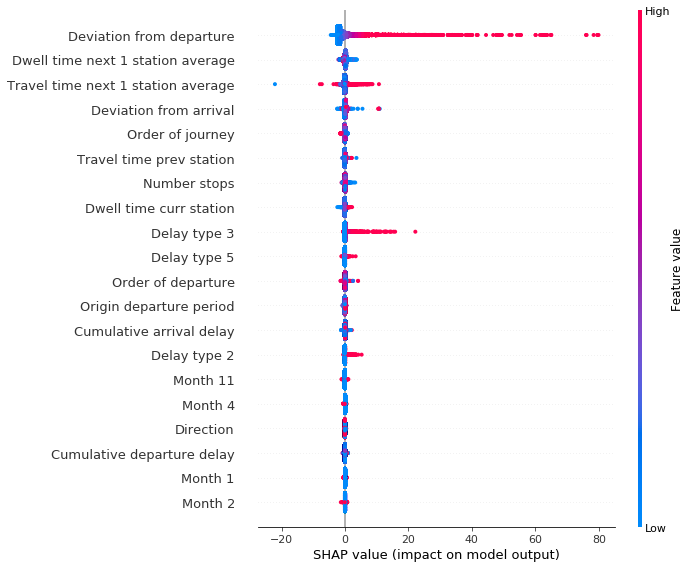
\includegraphics[width=0.5\textwidth]{Images/XGBoost_shap_evaluation/XGBoost_1_step_arr_dev_summary.png}\label{fig:1_step_arrival_deviation_summary}}
      \subfloat{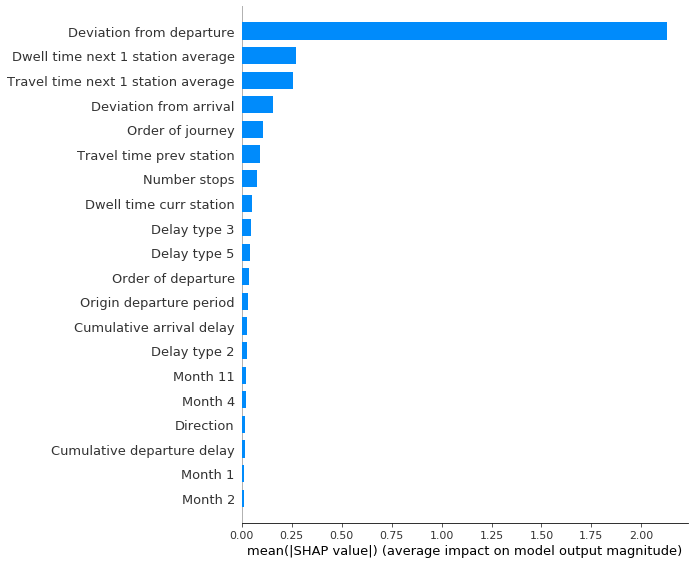
\includegraphics[width=0.5\textwidth]{Images/XGBoost_shap_evaluation/XGBoost_1_step_arr_dev_summary_bar.png}\label{fig:1_step_arrival_deviation_summary_bar}}
      \caption{1-step XGBoost arrival delay SHAP evaluation}
\end{figure}
\begin{figure}[H]
     \subfloat{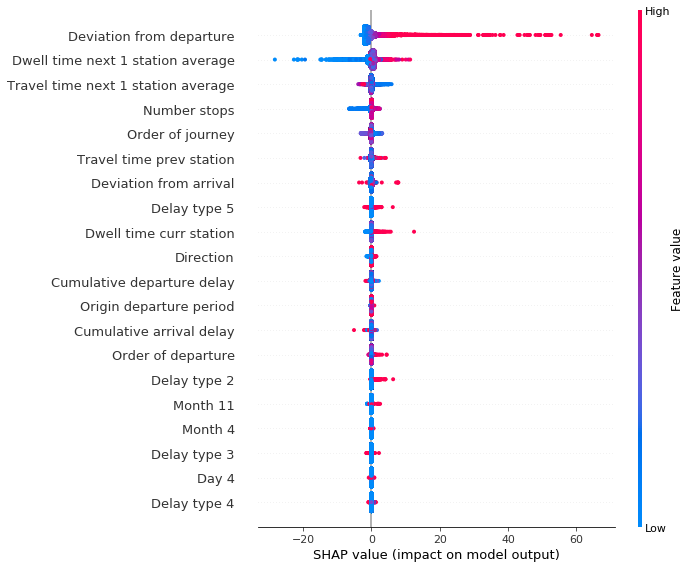
\includegraphics[width=0.5\textwidth]{Images/XGBoost_shap_evaluation/XGBoost_1_step_dep_dev_summary.png}\label{fig:1_step_depature_deviation_summary}}
     \subfloat{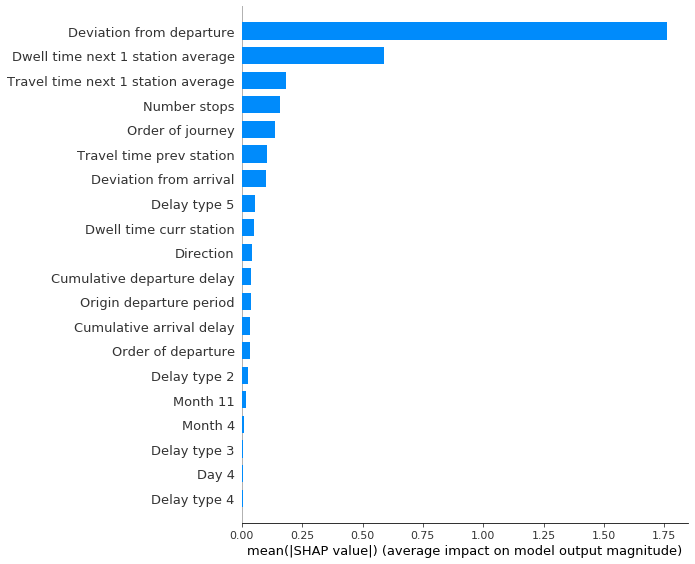
\includegraphics[width=0.5\textwidth]{Images/XGBoost_shap_evaluation/XGBoost_1_step_dep_dev_summary_bar.png}\label{fig:1_step_depature_deviation_summary_bar}}
     \caption{1-step XGBoost departure delay SHAP evaluation}
\end{figure}
\begin{figure}[H]
     \subfloat{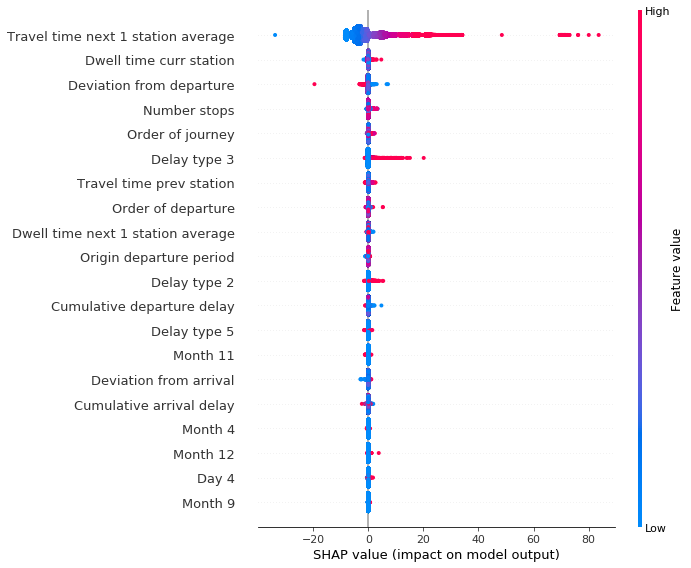
\includegraphics[width=0.5\textwidth]{Images/XGBoost_shap_evaluation/XGBoost_1_step_travel_time_summary.png}\label{fig:1_step_travel_time_summary}}
     \subfloat{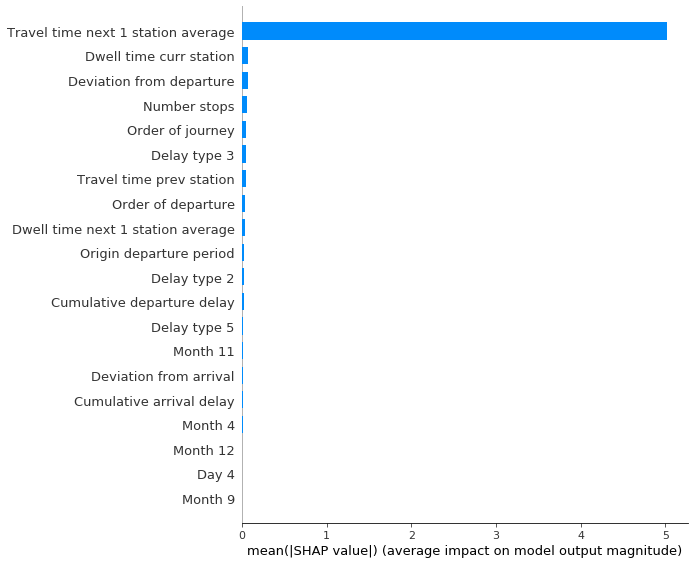
\includegraphics[width=0.5\textwidth]{Images/XGBoost_shap_evaluation/XGBoost_1_step_travel_time_summary_bar.png}\label{fig:1_step_travel_time_summary_bar}}
     \caption{1-step XGBoost travel time SHAP evaluation}
\end{figure}
\begin{figure}[H]
     \subfloat{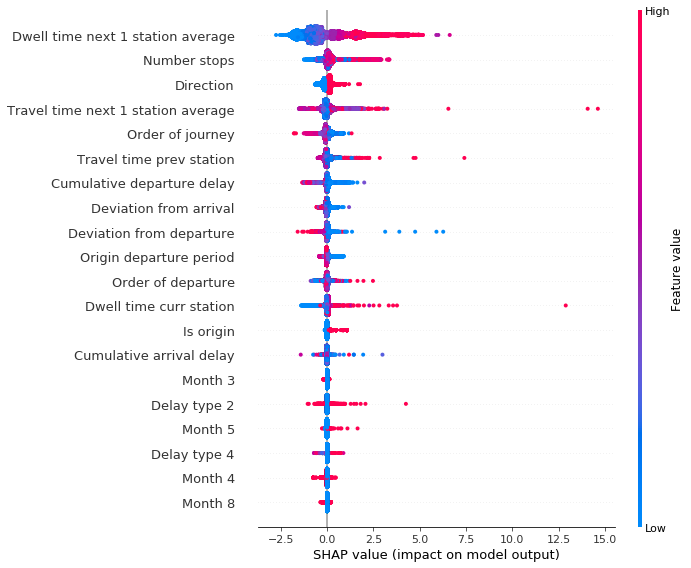
\includegraphics[width=0.5\textwidth]{Images/XGBoost_shap_evaluation/XGBoost_1_step_dwell_time_summary.png}\label{fig:1_step_dwell_time_summary}}
     \subfloat{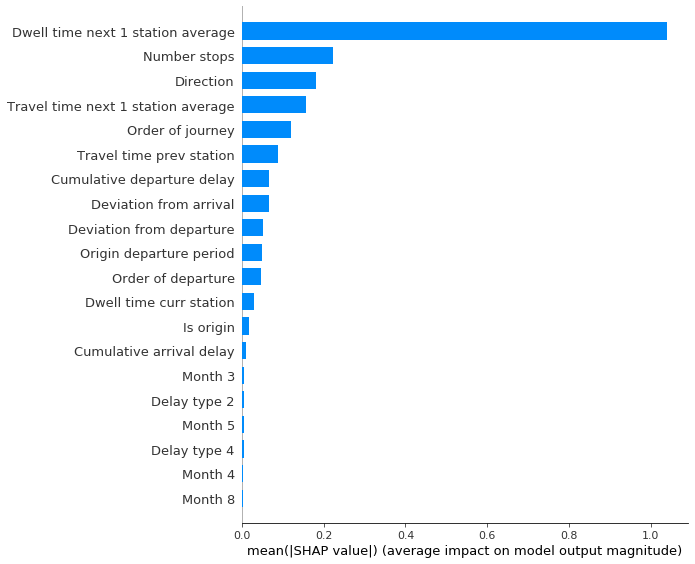
\includegraphics[width=0.5\textwidth]{Images/XGBoost_shap_evaluation/XGBoost_1_step_dwell_time_summary_bar.png}\label{fig:1_step_dwell_time_summary_bar}}
     \caption{1-step XGBoost dwell time SHAP evaluation}
     \label{fig:XGBoost_DNN_1_step_plot}
\end{figure}
\begin{figure}[H]
     \centering
     \subfloat{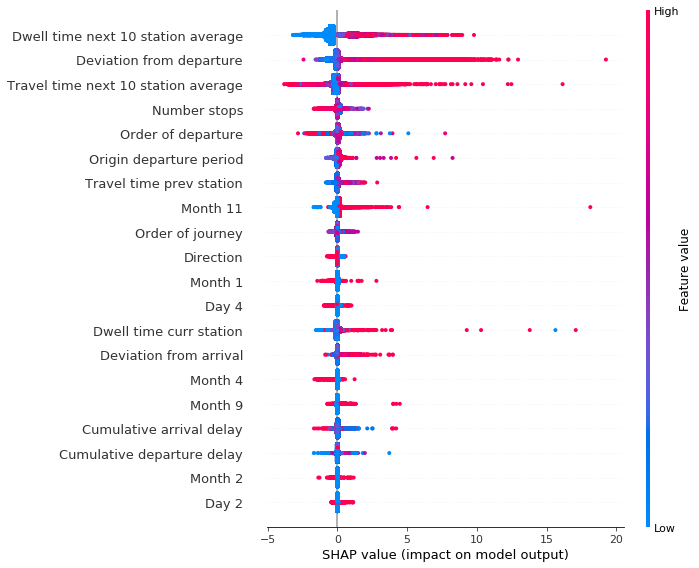
\includegraphics[width=0.5\textwidth]{Images/XGBoost_shap_evaluation/XGBoost_10_step_arr_dev_summary.png}\label{fig:10_step_arrival_deviation_summary}}
      \subfloat{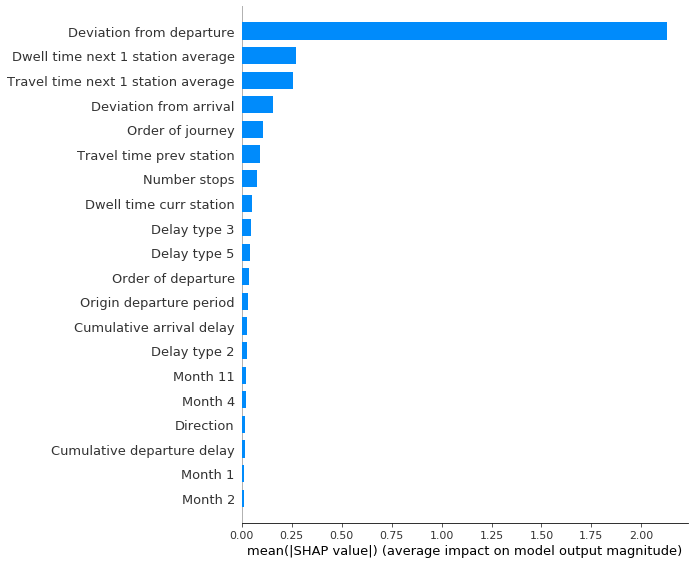
\includegraphics[width=0.5\textwidth]{Images/XGBoost_shap_evaluation/XGBoost_1_step_arr_dev_summary_bar.png}\label{fig:10_step_arrival_deviation_summary_bar}}
      \caption{10-step XGBoost arrival delay SHAP evaluation}
\end{figure}
\begin{figure}[H]
     \subfloat{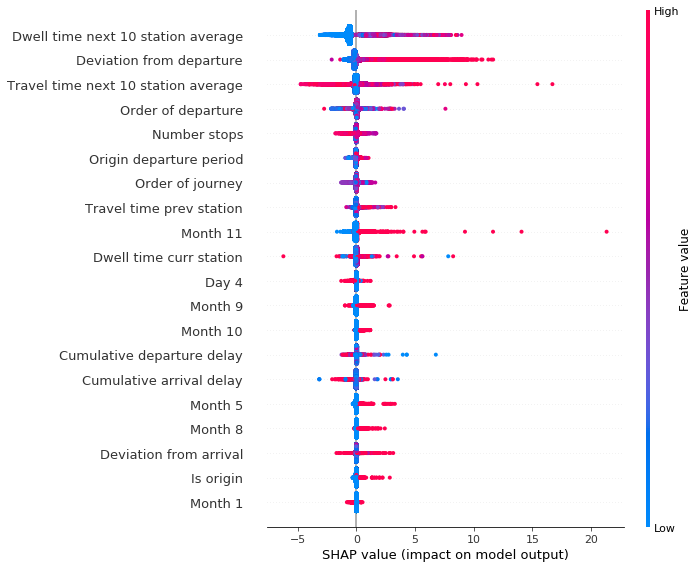
\includegraphics[width=0.5\textwidth]{Images/XGBoost_shap_evaluation/XGBoost_10_step_dep_dev_summary.png}\label{fig:10_step_depature_deviation_summary}}
     \subfloat{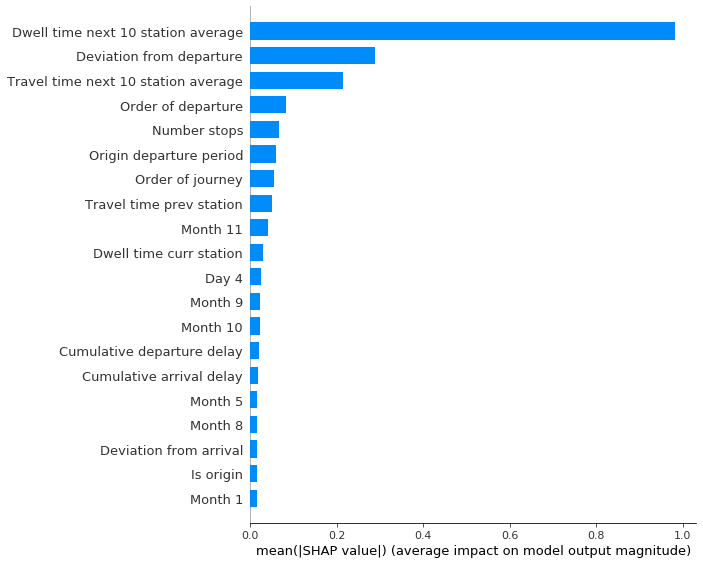
\includegraphics[width=0.5\textwidth]{Images/XGBoost_shap_evaluation/XGBoost_10_step_dep_dev_summary_bar.png}\label{fig:10_step_depature_deviation_summary_bar}}
     \caption{10-step XGBoost departure delay SHAP evaluation}
\end{figure}
\begin{figure}[H]
     \subfloat{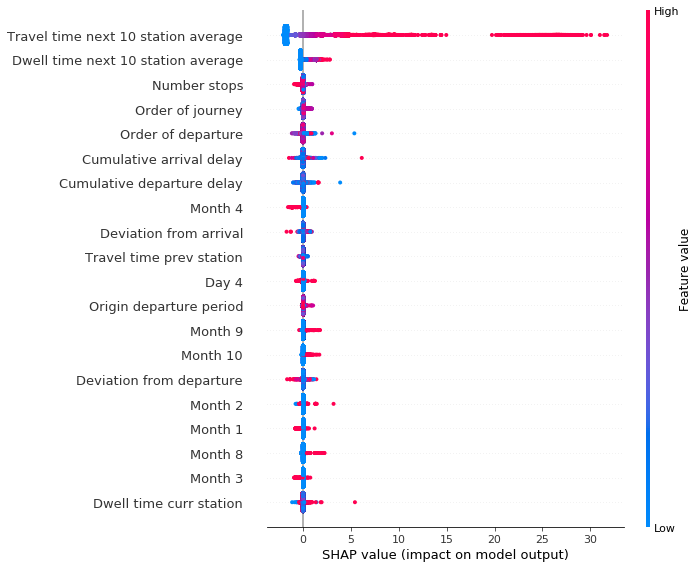
\includegraphics[width=0.5\textwidth]{Images/XGBoost_shap_evaluation/XGBoost_10_step_travel_time_summary.png}\label{fig:10_step_travel_time_summary}}
     \subfloat{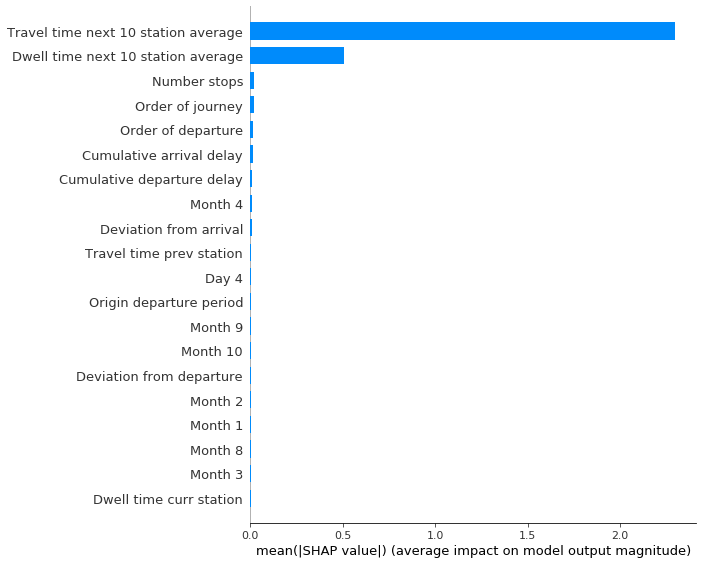
\includegraphics[width=0.5\textwidth]{Images/XGBoost_shap_evaluation/XGBoost_10_step_travel_time_summary_bar.png}\label{fig:10_step_travel_time_summary_bar}}
     \caption{10-step XGBoost travel time SHAP evaluation}
\end{figure}
\begin{figure}[H]
     \subfloat{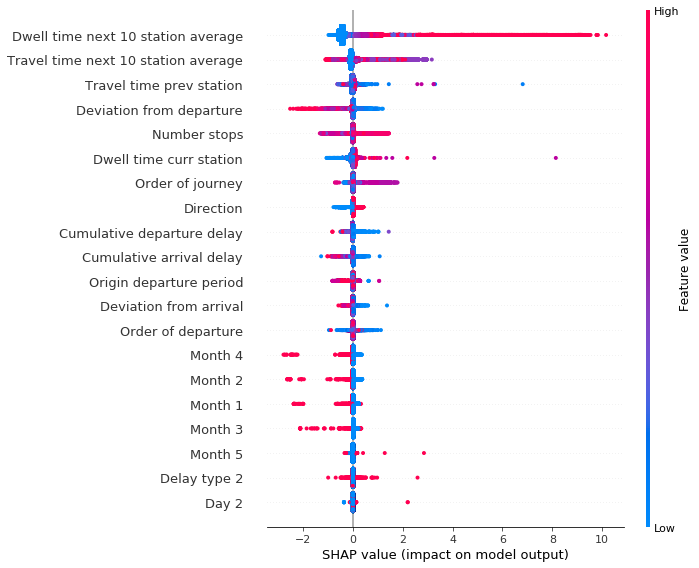
\includegraphics[width=0.5\textwidth]{Images/XGBoost_shap_evaluation/XGBoost_10_step_dwell_time_summary.png}\label{fig:10_step_dwell_time_summary}}
     \subfloat{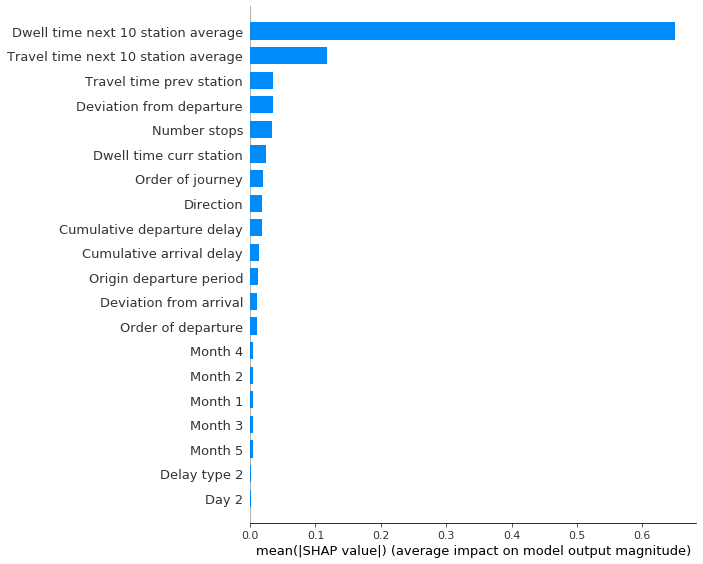
\includegraphics[width=0.5\textwidth]{Images/XGBoost_shap_evaluation/XGBoost_10_step_dwell_time_summary_bar.png}\label{fig:10_step_dwell_time_summary_bar}}
     \caption{10-step XGBoost dwell time SHAP evaluation}
     \label{fig:XGBoost_DNN_1_step_plot}
\end{figure}
As expected and shown in Figure \ref{fig:1_step_arrival_deviation_summary}, for the arrival deviation predictions, the most important features influencing the predictions are the deviation from scheduled departure (departure delay) of the trains previous station (delay propagation mechanism 1 - self propagation). There is consistency in high values of departure delay of trains from their previous station (red points) being associated with positive SHAP values up to a maximum value of approximately 80 and low values of departure delay of trains from their previous station (blue points) being associated with SHAP values close to zero. This allows us to conclude that the greater the departure delays of trains from their previous station, the greater the impact on the predicted deviation from scheduled arrival (arrival delay) of the train at the next station and in this specific case, the maximum contribution to the predicted arrival delay is 80 minutes. Interestingly, where they are greater than zero, delay propagation mechanism 3 (arrival forward delay propagation), 5 (departure forward delay propagation) and 2 (arrival backward delay propagation), consistently contribute positively to the arrival delay prediction whereas delay propagation mechanism 4 (departure backward delay propagation) does not contribute significantly to the arrival deviation predictions. Other than delay propagation mechanism 1 (self propagation), delay propagation 3 (arrival forward delay propagation) contributes the most out of all other delay propagation mechanisms as well as input variables. It could be naively deduced that other input variables, such as the average travel time, are significant in the arrival deviation prediction due to a high mean SHAP value. However, upon further inspection, there is no clear consistency to the SHAP values associated with each individual prediction i.e. a high average travel time, represented by red points, result in both positive and negative SHAP values, hence, suggesting that in this case, the average travel time feature is simply adding noise to the model. From Figure \ref{fig:1_step_depature_deviation_summary}, it can be deduced that the 1-step departure delay predictions are highly dependent upon both the departure delay from the train's previous station and the average dwell time of the train 1-step station ahead. This is intuitive as the dwell time of a train at any station should be fixed and therefore, the departure delay time is simply the dwell time in addition to the arrival delay. The most important features in the 1-step travel and dwell time predictions are the average 1-step travel time from checkpoint $C_i$ to $C_{i+1}$ and average dwell time at checkpoint $C_{i+1}$ respectively. This is testament to the fixed nature of these KPIs. It should be noted that the SHAP framework's local predictive capabilities explained in section \ref{Subsection:ModelInterpretability} are critical in formulating hypothesis for further testing. For example, as a result of the travel time SHAP evaluations, testing whether or not the average travel time from checkpoint $C_{i+q-1}$ to $C_{i+q}$ is sufficient on its own in the travel time prediction model should be undertaken as the global SHAP values are high for this feature and the local predictions of this feature are consistent, i.e. long average travel times from checkpoints $C_{i+q-1}$ to $C_{i+q}$ have high SHAP values and vice versa. On the other hand, for 10-step KPI predictions, through the SHAP analysis, average dwell time and travel time become much more important in the prediction. This is intuitive as long term delay will not be heavily influenced by immediate parameters therefore, general features such as average dwell time and travel time become much more important for the model to produce predictions.

\section{Concluding Remarks and Future Works}
In summary, in this paper, we demonstrated the superior KPI predictive capabilities and applicability of state-of-the-art ML techniques when coupled with vast data repositories as well as the improved understanding of delay propagation mechanisms through the SHAP framework.  The DNN and XGBoost models produced are able to provide more accurate real-time predictions of arrival delay, departure delay, travel times and dwell times compared to standard multiple linear regression, decision tree and industry's delay prediction system, Darwin. It is evident that through the SHAP framework the most important and pertinent delay propagation mechanisms, responsible for a reactionary delay, in the explored railway network are delay propagation mechanism 1 (self propagation), 3 (arrival forward delay propagation), 5 (departure forward delay propagation) and 2 (arrival backward delay propagation). 
Future extensions to this work include mapping out delay propagation chains throughout the network for improved visualisation and further understanding of large-scale network-wide cascading of delays. The models can also be improved through further utilizing the SHAP framework for data pruning. It would also be of interest to see whether the prediction of travel time and dwell time can be used to determine train arrival and departure times as well to determine delays, and whether delays derived in this manner is comparable to those predicted directly. To be able to summarize and evaluate model predictions in time-steps instead of steps as defined in the paper would also be of interest. Further statistical tests such as Granger's causality test alongside a model that reflects the structure of the network taking in order to capture relationships between various trains and therefore model the cascading delay effect throughout a network would also be an interesting extension to this work. Graphical neural networks (GNN) would be appropriate in this task where the vertices can represent the stations and the edges can represent movement of trains. Railway infrastructure data such as speed limits and signals can also be embedded into the GNN to provide further meaningful data. A combination of the SHAP framework and statistical tests such as the Granger's causality test should be utilized to optimize model performance through feature pruning and to provide statistical statements on what is the cause of any train delay at any time with what level of certainty. The ability to identify, connect and explain the combinations of primary and reactionary delays, as well as how they cascade throughout the network will be extremely useful in formulating appropriate counter-measures and maintenance schedules. 

\section*{Funding}
The work is supported by the key program project by Ministry of Science and Technology, China (grant no.2018YFB1600500), National Key Research and Development Project of China  (No. 2018AAA0101900), National Natural Science Foundation of China (U19B2042), Zhejiang University and Cybervein Joint Research Lab, Zhejiang Natural Science Foundation (LY19F020051). and also supported in part by the Zhejiang University/University of Illinois at Urbana-Champaign Institute, and was led by Principal Supervisor Simon Hu. 

\section*{Acknowledgements}
The authors would like to thank Yanfeng Ouyang at University of Illinois at Urbana-Champaign for his constructive feedback and stimulating discussions which ultimately led to the improvement of this paper. 

\newpage
\bibliographystyle{apacite}
\bibliography{bib1.bib}

\end{document}
